\setchapterpreamble[u]{\margintoc}

\chapter{The Evals Gap}
\labch{evals}

\epigraph{It doesn't matter how beautiful your theory is, \\
it doesn't matter how smart you are. \\
If it doesn't agree with experiment, it's wrong.}{Richard Feynman}

\section{Introduction}

The advent of LLMs marks a pivotal shift in the landscape of software development, testing and verification. Unlike traditional software systems, where deterministic outputs are the norm, LLMs introduce a realm of non-deterministic and generative behaviors that challenge conventional software engineering paradigms. This shift is not merely a technical evolution but a fundamental transformation in how we conceive, build, and assess software products.

For those entrenched in traditional methodologies, the transition to LLM-driven systems may seem daunting. However, ignoring this change is not an option. The reliance on outdated testing frameworks that fail to account for the probabilistic nature of LLMs will inevitably lead to significant setbacks.

To overcome these challenges, it is imperative to embrace the complexities of LLMs with a proactive mindset. This involves developing robust evaluation frameworks up-front that incorporate the generative nature of LLM-based software development while fostering a culture of continuous change, learning and adaptation.

\section{Non-Deterministic Generative Machines}

One of the most fundamental challenges when building products with LLMs is their generative and non-deterministic nature. Unlike traditional software systems where the same input reliably produces the same output, LLMs can generate novel text that may not exist in their training data, and produce different responses each time they're queried - even with identical prompts and input data. This behavior is both a strength and a significant engineering and product challenge.

When you ask an LLM the same question multiple times, you'll likely get different responses. This isn't a bug - it's a fundamental feature of how these models work. The ``temperature'' parameter, which controls the randomness of outputs, allows models to be creative and generate diverse responses. However, this same feature makes it difficult to build reliable, testable systems.

Consider a financial services company using LLMs to generate investment advice. The non-deterministic nature of these models means that:
\begin{itemize}
    \item The same input data could yield different analysis conclusions
    \item Regulatory compliance becomes challenging to guarantee
    \item User trust may be affected by inconsistent responses
    \item Testing becomes exceedingly more complex compared to traditional software
\end{itemize}

The primary source of non-determinism in LLMs comes from their sampling strategies. During text generation, the model:
\begin{enumerate}
    \item Calculates probability distributions for each next token
    \item Samples from these distributions based on temperature settings
    \item Uses techniques like nucleus sampling \sidecite{holtzman2020curiouscaseneuraltext} or top-k sampling to balance creativity and coherence
\end{enumerate}

In this simple experiment, we use an LLM to write a single-statement executive summary from an input financial filing. We observe that even a simple parameter like temperature can dramatically alter model behavior in ways that are difficult to systematically assess. At temperature $0.0$, responses are consistent but potentially too rigid. At $1.0$, outputs become more varied but less predictable. At $2.0$, responses can be wildly different and often incoherent. This non-deterministic behavior makes traditional software testing approaches inadequate.

\begin{minted}{python}
from dotenv import load_dotenv
import os

# Load environment variables from .env file
load_dotenv()

from openai import OpenAI
import pandas as pd
from typing import List

def generate_responses(
    model_name: str,
    prompt: str, 
    temperatures: List[float],
    attempts: int = 3
) -> pd.DataFrame:
    """
    Generate multiple responses at different temperature settings
    to demonstrate non-deterministic behavior.
    """
    client = OpenAI()
    results = []
    
    for temp in temperatures:
        for attempt in range(attempts):
            response = client.chat.completions.create(
                model=model_name,
                messages=[{"role": "user", "content": prompt}],
                temperature=temp,
                max_tokens=50
            )
            
            results.append({
                'temperature': temp,
                'attempt': attempt + 1,
                'response': response.choices[0].message.content
            })

    # Display results grouped by temperature 
    df_results = pd.DataFrame(results)
    for temp in temperatures:
        print(f"\nTemperature = {temp}")
        print("-" * 40)
        temp_responses = df_results[df_results['temperature'] == temp]
        for _, row in temp_responses.iterrows():
            print(f"Attempt {row['attempt']}: {row['response']}")
    
    return df_results
\end{minted}
% End of Selection


\begin{minted}{python}
MAX_LENGTH = 10000 # We limit the input length to avoid token issues
with open('../data/apple.txt', 'r') as file:
    sec_filing = file.read()

sec_filing
\end{minted}

\begin{figure}[h]
\centering
\includegraphics[width=0.7\textwidth]{evals/apple_sec.png}
\caption{Part of Apple Inc's SEC Filing. November 1, 2024 - 10-K: Annual report for year ending September 28, 2024}
\label{fig:apple-sec-temps}
\end{figure}


\begin{minted}{python}
MAX_LENGTH = 10000  # We limit the input length to avoid token issues
with open('../data/apple.txt', 'r') as file:
    sec_filing = file.read()
sec_filing = sec_filing[:MAX_LENGTH]
df_results = generate_responses(model_name="gpt-3.5-turbo",
                              prompt=f"Write a single-statement executive summary of the following text: {sec_filing}",
                              temperatures=[0.0, 1.0, 2.0])
\end{minted}

    
\begin{verbatim}
Temperature = 0.0
----------------------------------------
Attempt 1: Apple Inc. filed its Form 10-K for the fiscal year ended September 28, 2024 with the SEC, detailing its business operations and financial performance.
Attempt 2: Apple Inc. filed its Form 10-K with the SEC for the fiscal year ended September 28, 2024, detailing its business operations, products, and financial information.
Attempt 3: Apple Inc. filed its Form 10-K with the SEC for the fiscal year ended September 28, 2024, detailing its business operations, products, and financial information.

Temperature = 1.0
----------------------------------------
Attempt 1: Apple Inc., a well-known seasoned issuer based in California, designs, manufactures, and markets smartphones, personal computers, tablets, wearables, and accessories, with a focus on innovation and technology.
Attempt 2: Apple Inc. filed its Form 10-K with the SEC for the fiscal year ended September 28, 2024, reporting on its business operations, products, and financial performance.
Attempt 3: Apple Inc., a well-known seasoned issuer, filed its Form 10-K for the fiscal year ended September 28, 2024, reporting on its financial condition and operations.

Temperature = 2.0
----------------------------------------
Attempt 1: The Form 10-K for Apple Inc. for the fiscal year ended September 28, 2024, filed with the Securities and Exchange Commission, outlines the company's financial performance, products, and risk factors affecting future results.
Attempt 2: Apple Inc., a California-based company and leading technology manufacturer invDestacksmeticsisdiction setIspection-$20cyan evaluationseld anvisions droitEntering discernminerval Versbobprefversible vo该 Option和 meio forecast времCisco dellaischenpoihsCapabilities Geme.getTime future
Attempt 3: Apple Inc's Form 10-K provides a comprehensive overview of the company's financial reporting, business operations, products and market information.
\end{verbatim}

A temperature of 1 represents the unscaled probability scores for each token in the vocabulary. Decreasing the temperature closer to 0 sharpens the distribution, so the most likely token will have an even higher probability score. Conversely, increasing the temperature makes the distribution more uniform \sidecite{build-llms-from-scratch-book}:
\begin{itemize}
    \item Temperature = 0: Most deterministic, but potentially repetitive
    \item Temperature = 1: Balanced creativity and coherence 
    \item Temperature > 1: Increased randomness, potentially incoherent
\end{itemize}

How can one effectively test an LLM-powered system when the same prompt can yield radically different outputs based on a single parameter? Traditional testing relies on predictable inputs and outputs, but LLMs force us to grapple with probabilistic behavior. While lower temperatures may seem safer for critical applications, they don't necessarily eliminate the underlying uncertainty. This highlights the need for new evaluation paradigms that can handle both deterministic and probabilistic aspects of LLM behavior.

\section{Emerging Properties}

Beyond their non-deterministic nature, LLMs present another fascinating characteristic: emergent abilities that spontaneously arise as models scale up in size. These abilities - from basic question answering to complex reasoning - aren't explicitly programmed but rather emerge ``naturally'' as the models grow larger and are trained on more data. This makes evaluation fundamentally different from traditional software testing, where capabilities are explicitly coded and can be tested against pre-defined specifications.

Figure~\ref{fig:emerging-properties} provides a list of emergent abilities of large language models and the scale \sidecite{wei2022emergentabilitieslargelanguage}. The relationship between model scale and emergent abilities follows a fascinating non-linear pattern. Below certain size thresholds, specific abilities may be completely absent from the model - it simply cannot perform certain tasks, no matter how much you try to coax them out. However, once the model reaches critical points in its scaling journey, these abilities can suddenly manifest in what researchers call a phase transition - a dramatic shift from inability to capability. This unpredictable emergence of capabilities stands in stark contrast to traditional software development, where features are deliberately implemented and can be systematically tested.

\begin{figure}[h]
\centering
\includegraphics[width=0.6\textwidth]{evals/emerging.png}
\caption{Emergent abilities of large language models and the scale \cite{wei2022emergentabilitieslargelanguage}}
\label{fig:emerging-properties}
\end{figure}

The implications for evaluation are critical. While conventional software testing relies on stable test suites and well-defined acceptance criteria, LLM evaluation must contend with a constantly shifting landscape of capabilities. What worked to evaluate a 7B parameter model may be completely inadequate for a 70B parameter model that has developed new emergent abilities. This dynamic nature of LLM capabilities forces us to fundamentally rethink our approach to testing and evaluation.

\section{Problem Statement}

Consider a practical example that illustrates these challenges: building a Math AI tutoring system for children powered by an LLM. In traditional software development, you would define specific features (like presenting math problems or checking answers) and write tests to verify each function. But with LLMs, you're not just testing predefined features - you're trying to evaluate emergent capabilities like adapting explanations to a child's level, maintaining engagement through conversational learning, and providing age-appropriate safety-bound content.

This fundamental difference raises critical questions about evaluation:
\begin{itemize}
    \item How do we measure capabilities that weren't explicitly programmed?
    \item How can we ensure consistent performance when abilities may suddenly emerge or evolve?
    \item What metrics can capture both the technical accuracy and the subjective quality of responses?
\end{itemize}

The challenge becomes even more complex when we consider that traditional software evaluation methods simply weren't designed for these kinds of systems. There is an \textbf{Evals Gap} between traditional software testing and LLM evaluation. We need new frameworks that can account for both the deterministic aspects we're used to testing and the emergent properties that make LLMs unique. 

Table~\ref{evals-table} summarizes how LLM evaluation differs from traditional software testing across several key dimensions:
\begin{itemize}
    \item \textbf{Capability Assessment vs Functional Testing}: Traditional software testing validates specific functionality against predefined requirements. LLM evaluation must assess not necessarily pre-defined behavior but also ``emergent properties'' like reasoning, creativity, and language understanding that extend beyond explicit programming.

    \item \textbf{Metrics and Measurement Challenges}: While traditional software metrics can usually be precisely defined and measured, LLM evaluation often involves subjective qualities like ``helpfulness'' or ``naturalness'' that resist straightforward quantification. Even when we try to break these down into numeric scores, the underlying judgment often remains inherently human and context-dependent.

    \item \textbf{Dataset Contamination}: Traditional software testing uses carefully crafted test cases with known inputs and expected outputs (e.g., unit tests). In contrast, LLMs trained on massive internet-scale datasets risk having already seen and memorized evaluation examples during training, which can lead to artificially inflated performance scores. This requires careful dataset curation to ensure test sets are truly unseen by the model and rigorous cross-validation approaches.

    \item \textbf{Benchmark Evolution}: Traditional software maintains stable test suites over time. LLM benchmarks continuously evolve as capabilities advance, making longitudinal performance comparisons difficult and potentially obsoleting older evaluation methods.

    \item \textbf{Human Evaluation Requirements}: Traditional software testing automates most validation. LLM evaluation may demand significant human oversight to assess output quality, appropriateness, and potential biases through structured annotation and systematic review processes.
\end{itemize}

\begin{table}[h]
\caption{Evals of Traditional Software vs LLMs}
\label{evals-table}
\begin{tabular}{p{0.2\textwidth}p{0.35\textwidth}p{0.35\textwidth}}
\hline
\textbf{Aspect} & \textbf{Traditional Software} & \textbf{LLMs} \\
\hline
Capability Assessment & Validates specific functionality against requirements & May assess emergent properties like reasoning and creativity \\
\hline
Metrics and Measurement & Precisely defined and measurable metrics & Subjective qualities that resist straightforward quantification \\
\hline
Dataset Contamination & Uses carefully crafted test cases & Risk of memorized evaluation examples from training \\
\hline
Benchmark Evolution & Maintains stable test suites & Continuously evolving benchmarks as capabilities advance \\
\hline
Human Evaluation & Mostly automated validation & May require significant human oversight \\
\hline
\end{tabular}
\end{table}

\section{Evals Design}

A critical distinction must be made between evaluating an LLM versus evaluating an LLM-based application. While LLMs offer foundation capabilities and are typically general-purpose, LLM-based applications are more specific and tailored to particular use cases. An LLM-based application can be defined as a system that uses one or more LLMs to perform a specific task. More precisely, it represents the combination of one or more LLM models, their associated prompts and parameters configured to solve a particular business problem.

This differentiation significantly impacts the scope of evaluation. LLMs are typically evaluated based on their fundamental capabilities, including language understanding, reasoning and knowledge. In contrast, LLM-based applications should be evaluated based on their end-to-end functionality, performance, and how effectively they meet business requirements. This distinction carries several key implications for designing evaluation systems:

\begin{itemize}
    \item The same LLM can yield different results in different applications
    \item Evaluation must align with business objectives
    \item A great LLM does not guarantee a great application
\end{itemize}

Examples of key requirements for validation are listed in Table~\ref{validation-requirements}, ranging from Safety, Cognitive, Technical, Meta-Cognitive, to Ethical aspects.
The validation requirements for LLM applications span multiple critical categories, each with specific testing needs and importance:

\textbf{Safety Requirements}
\begin{itemize}
    \item \textbf{Misinformation Prevention}
    \begin{itemize}
        \item Testing needs: Factual accuracy verification, response consistency, hallucination detection, citation accuracy, uncertainty handling, temporal consistency, scientific accuracy
        \item Importance: Prevents real-world harm, maintains user trust, reduces legal risks, ensures reliable decision support
    \end{itemize}
    
    \item \textbf{Unqualified Advice Prevention}
    \begin{itemize}
        \item Testing needs: Recognition of professional queries, disclaimer consistency, referral mechanisms, boundary recognition, emergency handling
        \item Importance: Prevents harm from incorrect advice, reduces liability, protects vulnerable users
    \end{itemize}
    
    \item \textbf{Bias Detection}
    \begin{itemize}
        \item Testing needs: Gender/racial/cultural bias assessment, demographic representation, language inclusivity, stereotype avoidance
        \item Importance: Prevents bias reinforcement, ensures service equality, maintains social responsibility
    \end{itemize}
    
    \item \textbf{Privacy Protection}
    \begin{itemize}
        \item Testing needs: PII handling, data anonymization, information leakage prevention, compliance verification
        \item Importance: Protects confidentiality, ensures regulatory compliance, prevents breaches
    \end{itemize}
\end{itemize}

\textbf{Cognitive Requirements}
\begin{itemize}
    \item \textbf{Reasoning \& Logic}
    \begin{itemize}
        \item Testing needs: Problem-solving capability, mathematical accuracy, logical fallacy detection, causal reasoning
        \item Importance: Ensures reliable problem-solving, maintains computational accuracy
    \end{itemize}
    
    \item \textbf{Language Understanding}
    \begin{itemize}
        \item Testing needs: Context maintenance, idiom comprehension, cultural references, technical terminology
        \item Importance: Ensures effective communication, prevents misunderstandings
    \end{itemize}
\end{itemize}

\textbf{Technical Requirements}
\begin{itemize}
    \item \textbf{Code Generation}
    \begin{itemize}
        \item Testing needs: Syntax accuracy, security scanning, performance optimization, documentation quality
        \item Importance: Ensures code reliability, prevents security issues
    \end{itemize}
    
    \item \textbf{System Integration}
    \begin{itemize}
        \item Testing needs: API handling, rate limits, error management, response time, scalability
        \item Importance: Ensures system reliability, maintains performance
    \end{itemize}
\end{itemize}

\textbf{Meta-Cognitive Requirements}
\begin{itemize}
    \item \textbf{Self-Awareness}
    \begin{itemize}
        \item Testing needs: Knowledge limitation recognition, uncertainty communication, correction capabilities
        \item Importance: Builds trust, prevents overconfidence
    \end{itemize}
    
    \item \textbf{Communication Quality}
    \begin{itemize}
        \item Testing needs: Message clarity, audience appropriateness, information density
        \item Importance: Ensures understanding, maintains engagement
    \end{itemize}
\end{itemize}

\textbf{Ethical Requirements}
\begin{itemize}
    \item \textbf{Harmful Content Prevention}
    \begin{itemize}
        \item Testing needs: Content recognition, response appropriateness, filtering mechanisms
        \item Importance: Protects user safety, prevents misuse
    \end{itemize}
    
    \item \textbf{Decision-Making}
    \begin{itemize}
        \item Testing needs: Moral consistency, value alignment, fairness assessment
        \item Importance: Ensures ethical deployment, maintains standards
    \end{itemize}
\end{itemize}

\textbf{Environmental Requirements}
\begin{itemize}
    \item \textbf{CO2 Emission}
    \begin{itemize}
        \item Testing needs: Energy consumption monitoring, model efficiency, server optimization
        \item Importance: Reduces environmental impact, supports sustainability
    \end{itemize}
\end{itemize}



\section{Conceptual Overview}

Figure~\ref{fig:conceptual} demonstrates a conceptual design of key components of LLM Application evaluation.

\begin{figure}[h]
\centering
\includegraphics[width=0.4\textwidth]{evals/conceptual.png}
\caption{Conceptual overview of LLM-based application evaluation.}
\label{fig:conceptual}
\end{figure}
We observe three key components:

\textbf{1. Examples (Input Dataset)}
\begin{itemize}
    \item \textbf{Input:} Query to LLM App, e.g. user message, input file, image, audio, etc.
    \item \textbf{Output:} A reference expected outcome from the LLM application. Provide ground truth for comparison (\textit{Optional}).
    \item \textbf{Purpose:} Provides standardized test cases for evaluation.
\end{itemize}

\textbf{2. LLM Application (Processing Layer)}
\begin{itemize}
    \item \textbf{Input:} Test cases input from Examples
    \item \textbf{Output:} Generated responses/results
    \item \textbf{Purpose:}
    \begin{itemize}
        \item Represents different LLM implementations/vendors solving a specific task
        \item Could be different models (GPT-4, Claude, PaLM, etc.)
        \item Could be different configurations of same model
        \item Could be different prompting strategies
    \end{itemize}
\end{itemize}

\textbf{3. Evaluator (Assessment Layer)}
\begin{itemize}
    \item \textbf{Input:}
    \begin{itemize}
        \item Outputs from LLM application
        \item Reference data from Examples (\textit{Optional})
    \end{itemize}
    \item \textbf{Output:} Individual scores for target LLM application
    \item \textbf{Purpose:}
    \begin{itemize}
        \item Measures LLM Application performance across defined metrics
        \item Applies standardized scoring criteria
    \end{itemize}
\end{itemize}
Note that \textbf{Examples} must provide input data to the LLM Application for further evaluation. However, ground truth data is optional. We will return to this in more detail below, where we will see that ground truth data is not always available or practical. Additionally, there are approaches where one can evaluate LLM Applications without ground truth data.

A more general conceptual design is shown in Figure~\ref{fig:conceptual-multi}, where multiple LLM Applications are evaluated. This design allows for a more comprehensive evaluation of different configurations of LLM-based applications, e.g.:
\begin{itemize}
    \item Fixing all application parameters and evaluating different LLM models with their default configurations
    \item Fixing all parameters of an LLM model and evaluating different prompting strategies
\end{itemize}

\begin{figure}[h]
\centering
\includesvg[width=0.5\textwidth]{evals/conceptual-multi.svg}
\caption{Conceptual overview of Multiple LLM-based applications evaluation.}
\label{fig:conceptual-multi}
\end{figure}

In this evaluation framework, the same inputs are provided to all LLM applications, ensuring that responses are evaluated consistently. Performance is quantified objectively for each LLM Application, and results are ranked for easy comparison. This design leads to two additional components:
\textbf{4. Scores (Metrics Layer)}
\begin{itemize}
    \item \textbf{Input:} Evaluation results from Evaluator
    \item \textbf{Output:} Quantified performance metrics
    \item \textbf{Purpose:}
    \begin{itemize}
        \item Represents performance in numerical form
        \item Enables quantitative comparison among LLM applications
        \item May include multiple metrics per LLM application
    \end{itemize}
\end{itemize}

\textbf{5. Leaderboard (Ranking Layer)}
\begin{itemize}
    \item \textbf{Input:} Scores per LLM application
    \item \textbf{Output:} Ordered ranking of LLMs with scores
    \item \textbf{Purpose:}
    \begin{itemize}
        \item Aggregates and ranks performances across LLM applications
    \end{itemize}
\end{itemize}

\section{Design Considerations}
\subsection{Design Considerations}

The design of an LLM application evaluation system depends heavily on the specific use case and business requirements. Here we list important questions for planning an LLM application evaluation system pertaining to each of the key components previously introduced:

\textbf{1. Examples (Input Dataset):}
\begin{itemize}
    \item What types of examples should be included in the test set?
    \begin{itemize}
        \item Does it cover all important use cases?
        \item Are edge cases represented?
        \item Is there a good balance of simple and complex examples?
    \end{itemize}
    \item How do we ensure data quality?
    \begin{itemize}
        \item Are the examples representative of real-world scenarios?
        \item Is there any bias in the test set?
    \end{itemize}
    \item Should we have separate test sets for different business requirements?
    \item Do we need human-validated ground truth for all examples?
    \item Can we use synthetic data to augment the test set?
    \item How can business updates and user data be reflected in the dataset post-launch?
\end{itemize}

\textbf{2. LLM Applications:}
\begin{itemize}
    \item What aspects of each LLM app should be standardized for fair comparison?
    \begin{itemize}
        \item Prompt templates
        \item Context length
        \item Temperature and other parameters
        \item Rate limiting and timeout handling
    \end{itemize}
    \item What specific configurations impact business requirements?
    \begin{itemize}
        \item Which LLM application variations should be tested to maximize what we learn?
        \item Which LLM capabilities provide the most value for the business and how can we measure that?
    \end{itemize}
\end{itemize}

\textbf{3. Evaluator Design:}
\begin{itemize}
    \item How do we define success for different types of tasks?
    \begin{itemize}
        \item Task-specific evaluation criteria
        \item Objective metrics vs subjective assessment
    \end{itemize}
    \item Should evaluation be automated or involve human review?
    \begin{itemize}
        \item Balance between automation and human judgment
        \item Inter-rater reliability for human evaluation
        \item Cost and scalability considerations
    \end{itemize}
\end{itemize}

\textbf{4. Scoring System:}
\begin{itemize}
    \item How should different metrics be weighted?
    \begin{itemize}
        \item Relative importance of different factors
        \item Task-specific prioritization
        \item Business requirements alignment
    \end{itemize}
    \item Should scores be normalized or absolute?
    \item How to handle failed responses?
    \item Should we consider confidence scores from the LLMs?
\end{itemize}

\textbf{5. Leaderboard/Ranking:}
\begin{itemize}
    \item How often should rankings be updated?
    \item Should ranking include confidence intervals?
    \item How to handle ties or very close scores?
    \item Should we maintain separate rankings for different:
    \begin{itemize}
        \item Business requirements
        \item Model Cost Tiers
        \item LLM Model Families
    \end{itemize}
\end{itemize}

Holistically, your evaluation design should be built with scalability in mind to handle growing evaluation needs as the combination of (Input Examples X LLM Applications X Evaluators X Scores X Leaderboards) may grow very fast, particularly for an organization that promotes rapid experimentation and iterative development (good properties!). Finally, one should keep in mind that the evaluation system itself requires validation to confirm its accuracy and reliability vis-a-vis business requirements (evaluating evaluators will be later discussed in this Chapter).
\section{Metrics}

The choice of metric depends on the specific task and desired evaluation criteria. However, one can categorize metrics into two broad categories: \textbf{intrinsic} and \textbf{extrinsic}.

\begin{itemize}
    \item \textbf{Intrinsic metrics} focus on the model's performance on its primary training objective, which is typically to predict the next token in a sequence. Perplexity is a common intrinsic metric that measures how well the model predicts a given sample of text.

    \item \textbf{Extrinsic metrics} assess the model's performance on various downstream tasks, which can range from question answering to code generation. These metrics are not directly tied to the training objective, but they provide valuable insights into the model's ability to generalize to real-world applications.
\end{itemize}

Here, we are particularly interested in extrinsic metrics, since we are evaluating LLM-based applications rather than base LLM models.

Another way to think about metrics is in terms of the type of the task we evaluate:

\begin{enumerate}
    \item \textbf{Discriminative Task}:
    \begin{itemize}
        \item Involves distinguishing or classifying between existing data points.
        \item Examples: Sentiment analysis, classification, or identifying whether a statement is true or false.
    \end{itemize}
    
    \item \textbf{Generative Task}:
    \begin{itemize}
        \item Involves creating or producing new data or outputs.
        \item Examples: Text generation, image synthesis, or summarization.
    \end{itemize}
\end{enumerate}
For discriminative tasks, LLM-based applications may produce log-probabilities or discrete predictions, traditional machine learning metrics like accuracy, precision, recall, and F1 score can be applied. However, generative tasks may output text or images which require different evaluation approaches.

For generative tasks, a range of specialized metrics should be considered. These include match-based metrics such as exact match and prefix match, as well as metrics designed specifically for tasks like summarization and translation, including ROUGE, BLEU, and character n-gram comparisons. The selection of appropriate metrics should align with the specific requirements and characteristics of the task being evaluated.

In Table~\ref{tab:key-metrics} we provide a short list of widely used extrinsic metrics that can be used to evaluate generative tasks of LLM-based applications, along with their definitions, use cases, and limitations.
\begin{table}[htbp]
\caption{Key Metrics for Evaluating Generative Tasks}
\label{tab:key-metrics}
\begin{tabular}{p{0.2\textwidth}p{0.25\textwidth}p{0.25\textwidth}p{0.25\textwidth}}
\hline
\textbf{Metric} & \textbf{Definition} & \textbf{Use Case} & \textbf{Limitations} \\
\hline
\textbf{BLEU} (Bilingual Evaluation Understudy) & Measures overlap of n-grams between generated text and reference text & Machine translation and text summarization & \begin{itemize}\item Favors short outputs due to brevity penalty\item Insensitive to semantic meaning\item Requires high-quality reference texts\end{itemize} \\
\hline
\textbf{ROUGE} (Recall-Oriented Understudy for Gisting Evaluation) & Measures overlap between n-grams, words, or sentences of generated text and references, focusing on recall & Text summarization tasks & \begin{itemize}\item Biases toward long outputs\item Ignores semantic equivalence\item Heavily influenced by reference quality\end{itemize} \\
\hline
\textbf{METEOR} (Metric for Evaluation of Translation with Explicit ORdering) & Considers synonyms, stemming, and paraphrases alongside n-gram overlap & Machine translation, where semantic equivalence matters & \begin{itemize}\item Computationally expensive\item Subjective design of synonym/stemming databases\end{itemize} \\
\hline
\textbf{CIDEr} (Consensus-based Image Description Evaluation) & Measures n-gram overlap weighted by TF-IDF, tailored for image captioning & Image caption generation & \begin{itemize}\item Limited applicability outside captioning\item Heavily reliant on corpus statistics\end{itemize} \\
\hline
\textbf{TER} (Translation Edit Rate) & Computes number of edits needed to convert hypothesis into reference text & Translation quality evaluation & \begin{itemize}\item Doesn't consider semantic correctness\item Penalizes valid paraphrasing\end{itemize} \\
\hline
\textbf{BERTScore} & Uses contextual embeddings from pre-trained BERT to calculate token similarity & Tasks requiring semantic equivalence & \begin{itemize}\item High computational cost\item Performance varies with model used\end{itemize} \\
\hline
\textbf{SPICE} (Semantic Propositional Image Caption Evaluation) & Focuses on scene graphs in image captions to evaluate semantic content & Image captioning with emphasis on semantic accuracy & \begin{itemize}\item Designed only for image captions\item Less effective in purely textual tasks\end{itemize} \\
\hline
\end{tabular}
\end{table}
A common use case for metrics like BLEU and ROUGE is to evaluate the quality of generated summaries against reference summaries. To demonstrate this, consider the task of evaluating Financial Filings summaries against reference summaries (such as analyst-prepared highlights).

The simple metrics-based evaluator consists of several key components:
\begin{itemize}
    \item \textbf{Input:} Generated summary and reference summary
    \item \textbf{Output:} Dictionary containing scores for BLEU, ROUGE\_1, and ROUGE\_2
    \item \textbf{Purpose:} Evaluation of an LLM-based Financial Filings summary generator
\end{itemize}

A \textit{Reference Summary} represents the ``ideal'' summary, which may be prepared by human experts like analysts or generated by machines.

For this evaluation, the focus lies on comparing summaries generated by different LLM models of varying sizes and costs against a benchmark model. The evaluation setup uses:

\begin{itemize}
    \item \textbf{Benchmark model:} \texttt{gpt-4o}
    \item \textbf{Test models:} \texttt{gpt-4o-mini}, \texttt{gpt-4-turbo}, \texttt{gpt-3.5-turbo}
\end{itemize}

The core of the evaluation system is the \texttt{evaluate\_summaries} function, which calculates BLEU and ROUGE scores to assess text generation quality. This function accepts a generated summary and reference summary as input, processes them, and returns a dictionary containing three key metrics:
\begin{itemize}
    \item BLEU (measuring n-gram overlap)
    \item ROUGE\_1 (unigram comparison)
    \item ROUGE\_2 (bigram comparison)
\end{itemize}

This enables quantitative comparison of generated summaries against reference texts. The implementation utilizes HuggingFace's \texttt{evaluate} library to load and compute these metrics.
First, install the required Python packages:

\begin{minted}{bash}
pip install evaluate absl-py rouge_score
\end{minted}

The core evaluation function is implemented as follows:

\begin{minted}{python}
import evaluate
def evaluate_summaries(generated_summary, reference_summary):
    """
    Evaluate generated summaries against reference summaries using multiple metrics.
    
    Args:
        generated_summary (str): The summary generated by the model
        reference_summary (str): The reference/ground truth summary
        
    Returns:
        dict: Dictionary containing scores for different metrics
    """
    # Initialize metrics
    bleu = evaluate.load("google_bleu")
    rouge = evaluate.load("rouge")
    
    # Format inputs for BLEU (expects list of str for predictions and list of list of str for references)
    predictions = [generated_summary]
    references = [reference_summary]
    
    # Compute BLEU score
    bleu_score = bleu.compute(predictions=predictions, references=[references])
    
    # Compute ROUGE scores
    rouge_score = rouge.compute(predictions=predictions, references=references)
    
    # Compute Character metric    
    # Combine all scores into a single dictionary
    scores = {
        'bleu': bleu_score["google_bleu"],
        'rouge1': rouge_score['rouge1'],
        'rouge2': rouge_score['rouge2']
    }
    
    return scores
\end{minted}

For instance, \texttt{evaluate\_summaries} can be used to compare two arbitrary sentences and returns a dictionary with our chosen metrics:

\begin{minted}{python}
sentence1 = "the cat sat on the mat"
sentence2 = "the cat ate the mat" 
evaluate_summaries(sentence1, sentence2)
\end{minted}


\begin{verbatim}
    {'bleu': 0.3333333333333333,
     'rouge1': 0.7272727272727272,
     'rouge2': 0.4444444444444445}
\end{verbatim}


Next, we define \texttt{generate\_summary}, our simple LLM-based SEC filing summarizer application using OpenAI's API. It takes an arbitrary \texttt{model}, and an \texttt{input} text and returns the corresponding LLM's response with a summary.

\begin{minted}{python}
from openai import OpenAI
client = OpenAI()

def generate_summary(model, input):
    """
    Generate a summary of input using a given model
    """
    TASK = "Generate a 1-liner summary of the following excerpt from an SEC filing."

    prompt = f"""
    ROLE: You are an expert analyst tasked with summarizing SEC filings.
    TASK: {TASK}
    """
    
    response = client.chat.completions.create(
    model=model,
        messages=[{"role": "system", "content": prompt},
                 {"role": "user", "content": input}]
    )
    return response.choices[0].message.content
\end{minted}
Next, we define \texttt{evaluate\_summary\_models} - our benchmark evaluator - that compares text summaries generated by different language models against a benchmark model. The function:

\begin{enumerate}
    \item Takes a benchmark model, list of test models, prompt, and input text
    \item Generates a reference summary using the benchmark model and our \texttt{generate\_summary} function
    \item Generates summaries from all test models using \texttt{generate\_summary} function
    \item Evaluates each test model's summary against the benchmark using \texttt{evaluate\_summaries}
    \item Returns evaluation results and the generated summaries
\end{enumerate}

\begin{minted}{python}
def evaluate_summary_models(model_benchmark, models_test, input):
    """
    Evaluate summaries generated by multiple models
    """
    benchmark_summary = generate_summary(model_benchmark, input)

    # Generate summaries for all test models using list comprehension
    model_summaries = [generate_summary(model, input) for model in models_test]
    
    # Evaluate each model's summary against the benchmark
    evaluation_results = [evaluate_summaries(summary, benchmark_summary) for summary in model_summaries]

    return [evaluation_results, model_summaries, benchmark_summary]
\end{minted}

We are ready to run our benchmark evaluation. We define a benchmark model and a list of test models and then evaluate each test model's summary against the benchmark. We also print the generated summaries for each model.

\begin{minted}{python}
model_benchmark = "gpt-4o"
models_test = ["gpt-4o-mini", "gpt-4-turbo", "gpt-3.5-turbo"]

evals, model_summaries, benchmark_summary = evaluate_summary_models(model_benchmark, models_test, sec_filing)

print(benchmark_summary)
\end{minted}



    \begin{verbatim}
Apple Inc.'s 10-K filing for the fiscal year ending September 28, 2024, outlines its operational and financial condition, detailing the company's diverse product lines, market activities, and compliance with SEC requirements.
    \end{verbatim}



\begin{minted}{python}
# Print each model name and its summary
for model, summary in zip(models_test, model_summaries):
    print(f"{model}: \n {summary} \n---------------")
\end{minted}

\begin{verbatim}
gpt-4o-mini: 
 Apple Inc. filed its Annual Report on Form 10-K for the fiscal year ending September 28, 2024, detailing its business operations, risks, and financial condition. 
---------------
gpt-4-turbo: 
 Apple Inc.'s Form 10-K for the fiscal year ended September 28, 2024, details its annual report as a well-known seasoned issuer, confirming compliance with SEC regulations and reporting on stock performances, securities, and corporate governance, while also including forward-looking statements subject to various risks. 
---------------
gpt-3.5-turbo: 
 Apple Inc. filed its Form 10-K with the SEC, revealing financial information for the fiscal year ended September 28, 2024, including details on its products and market performance. 
---------------
\end{verbatim}


The benchmark summary from \texttt{gpt-4o} provides a balanced overview of the analyzed excerpt from Apple's 10-K filing, focusing on operational status, financial condition, product lines, and regulatory compliance.

When comparing our test models against the benchmark, we observe that \texttt{gpt-4o-mini} provides a concise yet comprehensive summary that closely aligns with the benchmark's core message. While it omits product lines, it effectively captures the essential elements of the filing including business operations, risks, and financial condition. Its brevity and focus look (subjectively) similar to our benchmark model.

\texttt{gpt-4-turbo} performs adequately but tends toward verbosity. While it includes relevant information about SEC compliance, it introduces peripheral details about seasoned issuer status and forward-looking statements. The additional complexity makes the summary less focused than \texttt{gpt-4o-mini}'s version.

\texttt{gpt-3.5-turbo} looks quite different from the benchmark. Its summary, while factually correct, is overly simplified and misses key aspects of the filing. The model captures basic financial information but fails to convey the breadth of operational and compliance details present in the benchmark summary.

Of course, the above evaluation is only based on a single example and is heavily subjective. It's a ``vibe check'' on our evaluation results. Now, for an objective analysis, we can look at the quantitative metrics we have chosen and use the \texttt{visualize\_prompt\_comparison} function we write below to visualize the performance of our test models across our predefined quantitative metrics.

\begin{minted}{bash}
pip install matplotlib
\end{minted}

\begin{minted}{python}
def visualize_prompt_comparison(evaluation_results, model_names):
    """
    Create a radar plot comparing different prompt variations
    
    Args:
        evaluation_results (list): List of dictionaries containing evaluation metrics
        model_names (list): List of names for each prompt variation
    """
    from evaluate.visualization import radar_plot
    
    # Format data for visualization
    plot = radar_plot(data=evaluation_results, model_names=model_names)
    return plot

# Create and display visualization
plot = visualize_prompt_comparison(evals, models_test)
plot.show()
\end{minted}


\begin{figure}[h]
\centering
\includegraphics[width=0.8\textwidth]{evals/evals_30_1.png}
\caption{Radar plot comparing model performance across evaluation metrics}
\label{fig:model_comparison}
\end{figure}

Results demonstrate that tested models perform quite differently on our predefined metrics. The evaluation metrics puts \texttt{gpt-4o-mini} as the closest aligned to the benchmark, followed by \texttt{gpt-4-turbo}, and \texttt{gpt-3.5-turbo} showing the largest deviation. This suggests that \texttt{gpt-4o-mini} is the best model for this task at least on the metrics we have chosen and for the set of models we have tested.

While evaluating language model outputs inherently involves subjective judgment, establishing a high-quality benchmark model and using quantifiable metrics provide a more objective framework for comparing model performance. This approach transforms an otherwise qualitative assessment into a measurable, data-driven evaluation process.

These metrics provide quantifiable measures of performance, however limitations should be mentioned:

\begin{itemize}
    \item \textbf{Task-specific nature}: Chosen set of metrics might not fully capture the nuances of complex generative-based tasks, especially those involving subjective human judgment.
    \item \textbf{Sensitivity to data distribution}: Performance on these metrics can be influenced by the specific dataset used for evaluation, which might not represent real-world data distribution.
    \item \textbf{Subjective Acceptable Threshold}: These metrics are not always easy to interpret and set a threshold for (see \sidecite{sarmah2024choosethresholdevaluationmetric} for a discussion on how to choose a threshold for an evaluation metric for large language models).
    \item \textbf{Inability to assess reasoning or factual accuracy}: These metrics primarily focus on surface-level matching and might not reveal the underlying reasoning process of the LLM or its ability to generate factually correct information.
\end{itemize}

In conclusion, selecting an appropriate extrinsic metrics set depends on the specific task, underlying business requirements and desired evaluation granularity. Understanding the limitations of these metrics can provide a more comprehensive assessment of LLM performance in real-world applications.

To address these limitations, alternative approaches like \textbf{human-based evaluation} and \textbf{model-based evaluation} are often used, which will be discussed in the following sections.
\section{Evaluators}

\subsection{Model-Based Evaluation}
\label{sec:model-based-eval}
Traditional metrics like BLEU or ROUGE often fall short in capturing the nuanced, contextual, and creative outputs of LLMs. As an alternative we can consider a ``Model-based evaluation'' approach. A common approach is to use an LLM as a judge. This is an approach that leverages language models themselves to assess the quality of outputs from other language models. This method involves using a model (often a more capable one) to act as an automated judge, evaluating aspects like accuracy, coherence, and relevance of generated content. Unlike traditional metrics that rely on exact matching or statistical measures, model-based evaluation can capture nuanced aspects of language and provide more contextual assessment.

As discussed in the paper \sidecite{li2024leveraginglargelanguagemodels}, LLM-based evaluation approaches generally fall into two main categories:

\begin{enumerate}
    \item \textbf{Prompt-based evaluation}: This involves using prompts to instruct existing LLMs to evaluate text quality without any fine-tuning. The evaluation can take several forms:
    \begin{itemize}
        \item Score-based: LLMs assign numerical scores to generated text
        \item Probability-based: Using generation probability as a quality metric
        \item Likert-style: Rating text quality on discrete scales
        \item Pairwise comparison: Directly comparing two texts
        \item Ensemble methods: Combining multiple LLM evaluators
    \end{itemize}
    \item \textbf{Tuning-based evaluation}: This involves fine-tuning open-source LLMs specifically for evaluation tasks. This can be more cost-effective than repeatedly using API calls and allows for domain adaptation.
\end{enumerate}

Once you have chosen your approach, a general LLM-as-a-Judge procedure involves the following steps (see Figure~\ref{fig:llm_judge}):
\begin{enumerate}
    \item \textbf{Define Evaluation Criteria}: Establish clear benchmarks, such as relevance, coherence, accuracy, and fluency.
    \item \textbf{Prepare Prompts}: Craft effective prompts to guide the LLM in evaluating content against the criteria.
    \item \textbf{Define Reference Data}: Establish a set of reference data that the judge model can use to evaluate the generated outputs. (\textit{Optional})
    \item \textbf{Run Evaluations}: Use the judge model to score outputs. Consider using a large and/or more capable model as a judge to provide more nuanced assessments.
    \item \textbf{Aggregate and Analyze Results}: Interpret scores to refine applications.
\end{enumerate}
\begin{figure}[h]
\centering
\includesvg[width=0.6\textwidth]{evals/llm_judge.svg}
\caption{Conceptual overview of LLM-as-a-Judge evaluation.}
\label{fig:llm_judge}
\end{figure}

Compared to traditional metrics, LLM-as-a-Judge evaluation offers a more sophisticated assessment framework by leveraging natural language criteria. While metrics focus on statistical measures, judge models excel at evaluating subjective qualities such as creativity, narrative flow, and contextual relevance - aspects that closely mirror human judgment. The judge model processes evaluation guidelines expressed in natural language, functioning similarly to a human reviewer interpreting assessment criteria. One notable consideration is that this approach requires careful prompt engineering to properly define and communicate the evaluation standards to the model.

Prompt Engineering can have a large impact on the quality of the evaluation \sidecite{li2024leveraginglargelanguagemodels}. Hence, it's worth noting key prompting best practices when designing LLM-as-a-judge evaluators \sidecite{huggingface2024llmjudge}:
\begin{enumerate}
    \item Use discrete integer scales (e.g., 1-5) rather than continuous ranges 
    \item Provide clear rubrics that define what each score level means
    \item Include reference answers when available to ground the evaluation
    \item Break down complex judgments into specific evaluation criteria
\end{enumerate}

Additionally, the interpretability of the evaluation framework can be fostered by:
\begin{enumerate}
    \item Requiring explanations and reasoning for scores to increase transparency 
    \item Having a hollistic evaluation by considering multiple dimensions such as coherence, relevance, and fluency
\end{enumerate}
Below we provide a sample implementation of an LLM-as-a-Judge evaluation system for our LLM application that generates SEC filing summaries. The code defines:

\begin{enumerate}
    \item A \texttt{JudgeEvaluation} Pydantic model that enforces type validation for four key metrics:
    \begin{itemize}
        \item \textbf{Expertise}: Rating of analyst-level writing quality
        \item \textbf{Coherence}: Score for logical organization  
        \item \textbf{Fluency}: Assessment of grammar and clarity
        \item \textbf{Similarity}: Measure of alignment with reference text
    \end{itemize}

    \item An \texttt{evaluate\_with\_llm()} function that:
    \begin{itemize}
        \item Takes a judge model, candidate summary, and reference summary as inputs
        \item Constructs a detailed prompt instructing the LLM to act as an expert evaluator
        \item Uses structured output parsing to return scores in a consistent format
        \item Returns scores on a 1-10 scale for each evaluation criterion
    \end{itemize}
\end{enumerate}

The implementation demonstrates how to combine structured data validation with natural language evaluation to create a robust automated assessment system.

\begin{minted}{python}
from pydantic import BaseModel
from typing import List, Dict

class JudgeEvaluation(BaseModel):
    expertise: int
    coherence: int
    fluency: int
    similarity: int
def evaluate_with_llm(judge_model: str, candidate_summary: str, reference_summary: str) -> Dict[str, float]:
    """
    Use an LLM to evaluate a candidate summary against a reference summary.
    
    Args:
        judge_model (str): Name of the model to use as the judge.
        candidate_summary (str): Generated summary to evaluate.
        reference_summary (str): Ground truth or benchmark summary.
    
    Returns:
        dict: Dictionary containing evaluation scores for specified criteria.
    """
    prompt = f"""
    ROLE: You are an expert evaluator of SEC Filing summaries. Evaluate the following candidate summary against the reference summary on a scale of 1 to 10 for the following criteria:
    - Expertise: Does the summary look like it was written by an expert analyst?
    - Coherence: Is the candidate summary logically organized and easy to understand?
    - Fluency: Is the language of the candidate summary clear and grammatically correct?
    - Similarity: How similar is the candidate summary compared to the reference summary?

    Reference Summary:
    "{reference_summary}"

    Candidate Summary:
    "{candidate_summary}"

    Provide scores in this format:
    Expertise: X, Coherence: Y, Fluency: Z, Similarity: W
    """
    completion = client.beta.chat.completions.parse(
        model=judge_model,
        messages=[{"role": "system", "content": prompt}],
        response_format=JudgeEvaluation
    )
    return completion.choices[0].message.parsed
\end{minted}
Next, we define an \texttt{evaluate\_summary\_models} function that leverages our LLM-as-a-Judge function to compare summaries generated by different language models. The function works in three steps:

First, it generates a benchmark summary using the specified benchmark model. Then, it generates summaries using each of the test models. Finally, it evaluates each test model's summary against the benchmark using the judge model.

As a result, we get a list of evaluation results we can use to compare our candidate LLM models across our predefined metrics.

\begin{minted}{python}
def evaluate_summary_models(judge_model: str, benchmark_model: str, test_models: List[str], input_text: str):
    """
    Evaluate summaries generated by multiple models using an LLM-as-a-Judge approach.
    
    Args:
        judge_model (str): Name of the model to use as the judge.
        benchmark_model (str): Name of the benchmark model.
        test_models (list): List of model names to test.
        input_text (str): Input text for summarization.
    
    Returns:
        tuple: Evaluation results, model summaries, benchmark summary.
    """
    benchmark_summary = generate_summary(benchmark_model, input_text)
    model_summaries = [generate_summary(model, input_text) for model in test_models]

    evaluation_results = [
        evaluate_with_llm(judge_model, summary, benchmark_summary)
        for summary in model_summaries
    ]

    return evaluation_results, model_summaries, benchmark_summary
\end{minted}

\begin{minted}{python}
# Example Usage
model_benchmark = "gpt-4o"
models_test = ["gpt-4o-mini", "gpt-4-turbo", "gpt-3.5-turbo"]
judge_model = "gpt-4o"

evals, model_summaries, benchmark_summary = evaluate_summary_models(
    judge_model, model_benchmark, models_test, sec_filing
)
\end{minted}
Here, we can see the benchmark summary coming from our benchmark model \texttt{gpt-4o}:

\begin{minted}{python}
benchmark_summary
\end{minted}


    \begin{verbatim}
    "Apple Inc.'s annual report for the fiscal year ending September 28, 2024, details its business operations, financial condition, and product lines, including iPhones, Macs, iPads, and wearables, and incorporates forward-looking statements regarding its future performance."
    \end{verbatim}


Next, we obtain the summaries and evaluation results generated by our test models, \texttt{gpt-4o-mini}, \texttt{gpt-4-turbo} and \texttt{gpt-3.5-turbo}, respectively.

\begin{minted}{python}
model_summaries
\end{minted}



    \begin{verbatim}
    ['Apple Inc. filed its annual Form 10-K report for the fiscal year ended September 28, 2024, detailing its business operations, product lines, and financial performance.',
     "This Form 10-K filing by Apple Inc. for the fiscal year ended September 28, 2024, is an annual report detailing the company's financial performance, including registered securities, compliance with SEC reporting standards, and contains sections on business operations, risk factors, financial data, and management analysis.",
     'Apple Inc., a California-based technology company, reported an aggregate market value of approximately $2.6 trillion held by non-affiliates, with 15.1 billion shares of common stock outstanding as of October 18, 2024.']
    \end{verbatim}


As a result, we obtain a list of objects from the defined \texttt{JudgeEvaluation} Pydantic class which contains the evaluation metrics: expertise, coherence, fluency and similarity.

\begin{minted}{python}
evals
\end{minted}

\begin{verbatim}
[JudgeEvaluation(expertise=7, coherence=8, fluency=8, similarity=7),
 JudgeEvaluation(expertise=7, coherence=7, fluency=8, similarity=5),
 JudgeEvaluation(expertise=4, coherence=5, fluency=7, similarity=2)]
\end{verbatim}


\begin{minted}{python}
# Convert evaluation objects to dictionaries
evals_list = [
    {
        "expertise": eval.expertise,
        "coherence": eval.coherence, 
        "fluency": eval.fluency,
        "similarity": eval.similarity
    }
    for eval in evals
]

# Visualize results
plot = visualize_prompt_comparison(evals_list, models_test)
plot.show()
\end{minted}



\begin{figure}[h]
\centering
\includegraphics{evals/evals_46_1.png}
\caption{Evaluation metrics comparison across test models}
\label{fig:eval-comparison}
\end{figure}

Analyzing the evaluation results across our test models (\texttt{gpt-4o-mini}, \texttt{gpt-4-turbo}, \texttt{gpt-3.5-turbo}), several interesting patterns emerge:

The \texttt{gpt-4o-mini} model demonstrated strong performance, achieving high scores across all metrics (expertise: 7, coherence: 8, fluency: 8, similarity: 7). This performance suggests it maintained robust quality despite being a smaller variant of our benchmark model \texttt{gpt-4o}.

The \texttt{gpt-4-turbo} model exhibited comparable expertise and fluency scores (7 and 8 respectively) but showed slightly reduced coherence (7) and notably lower similarity (5) compared to the benchmark. These results could indicate some divergence from the reference summary while maintaining overall quality.

The \texttt{gpt-3.5-turbo} model recorded the lowest scores (expertise: 4, coherence: 5, fluency: 7, similarity: 2), with particular weaknesses in expertise and similarity to the benchmark. While maintaining acceptable fluency, the marked decrease in similarity score indicates substantial deviation from the reference summary.

Figure \ref{fig:eval-comparison} illustrates these differences across models and evaluation dimensions. A distinct performance gradient can be observed from \texttt{gpt-4o-mini} to \texttt{gpt-3.5-turbo}, with the latter exhibiting significant degradation across most metrics.
Leveraging LLMs for evaluation has several limitations \sidecite{li2024leveraginglargelanguagemodels}. Firstly, computational overhead should not be neglected given the inherent cost of running additional model inferences iterations. LLM evaluators can also exhibit various biases, including order bias (preferring certain sequence positions), egocentric bias (favoring outputs from similar models), and length bias. Further, there may be a tight dependency on prompt quality - small prompt variations may lead to substantially different outcomes. It is important to also note challenges around domain-specific evaluation in fields such as medicine, finance, law etc, where a general llm-as-a-judge approach may not be suitable.

The LLM-as-a-Judge strategy can serve as a scalable and nuanced solution to evaluate LLM-based applications. While it does not entirely replace metrics-based or human-based approaches, it significantly augments evaluation workflows, especially in scenarios requiring evaluation of generative outputs. Future improvements in our example include integrating human oversight and refining LLMs for domain-specific evaluation tasks.

One open source solution trying to overcome some of these challenges is Glider \sidecite{deshpande2024glidergradingllminteractions}, a 3B evaluator LLM that can score any text input and associated context on arbitrary user defined criteria. Glider is an LLM model trained on 685 domains and 183 criteria whose judgement scores show $91.3\%$ agreement with human judgments, making it suitable for a diverse range of real world applications.

\section{Evaluating Evaluators}

We have discussed how LLMs can be used to evaluate LLM-based aplications. However, how can we evaluate the performance of LLMs that evaluate other LLMs? This is the question that meta evaluation aims to answer. Clearly, the discussion can become quite meta as we need to evaluate the performance of the evaluator to evaluate the performance of the evaluated model. However, one can make a case for two general options:

\begin{enumerate}
    \item Use a golden-standard dataset that is used to evaluate the performance of LLM evaluators using a ``metrics-based'' approach.
    \item Use a human evaluator to generate reference scores that can be used to evaluate the performance of the LLM evaluator (similar to the human-based evaluation we discussed earlier).
\end{enumerate}
As depicted in Figure~\ref{fig:meta}, the performance of the LLM evaluator can be evaluated by comparing its scores to either a golden-standard dataset or human reference scores. Higher correlation values indicate better performance of the LLM evaluator. For instance, if we were to evaluate the performance of a LLM-as-a-judge evaluator, in the task of evaluating multilingual capability of an LLM:
\begin{enumerate}
    \item In a ``metrics-based'' approach, we would first need to define a set of metrics that capture the task of multilingual capability. For instance, we could use the BLEU metric to evaluate the quality of the generated LLM output against a golden dataset (e.g. machine translated text). We would then calculate the correlation between these scores against those generated by the LLM evaluator. The higher the correlation, the better the LLM evaluator.
    \item In a ``human-based'' approach, we would need to recruit human evaluators that are experts in the target languages we are evaluating. Expert humans would provide scores for a set of samples of the input LLM. We would then calculate the correlation between these scores against those generated by the LLM evaluator. The higher the correlation, the better the LLM evaluator.
\end{enumerate}

\begin{figure}[h]
\centering
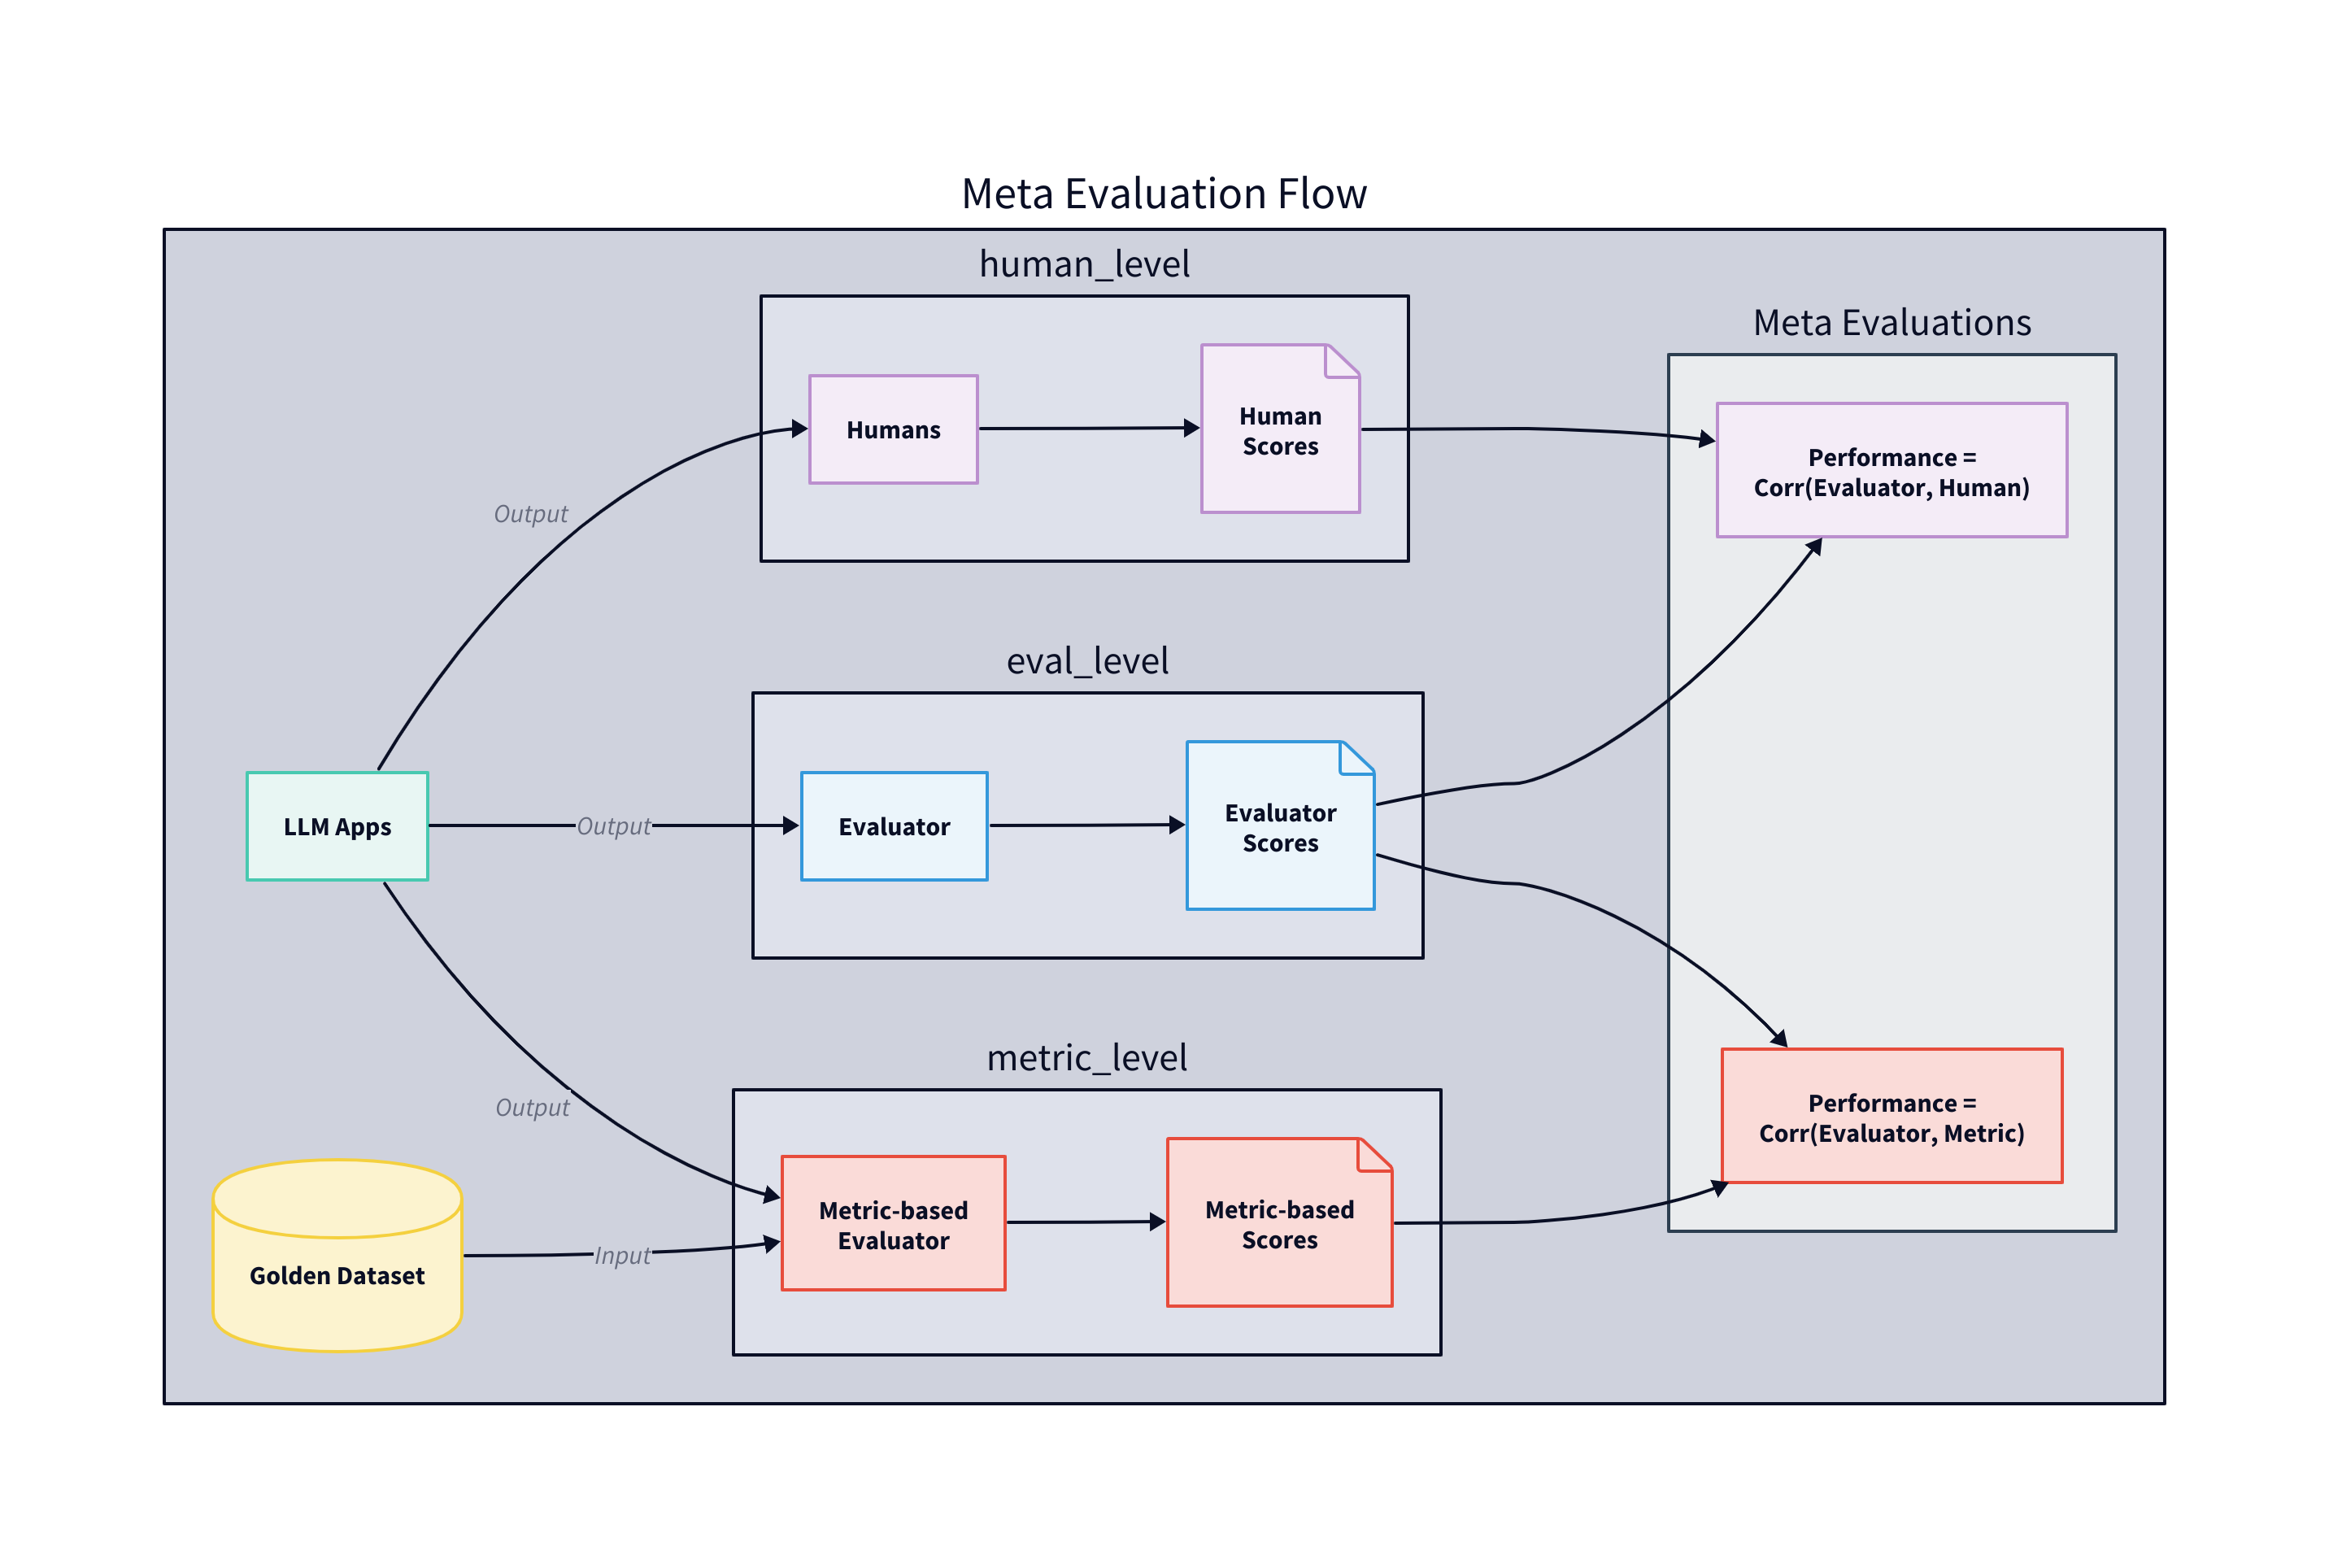
\includegraphics{evals/meta.png}
\caption{Conceptual overview of LLMs Meta Evaluation}
\label{fig:meta}
\end{figure}
An alternative to the above approaches is to use humans to directly evaluate the LLM-judges themselves. A notable example of this is Judge Arena \sidecite{judgearena2024}, which is a platform that allows users to vote on which AI model made the better evaluation. Under this approach, the performance of the LLM evaluator is given by the (blind) evaluation of humans who perform the voting on randomly generated pairs of LLM judges as depicted in Figure~\ref{fig:meta2}. Only after submitting a vote, users can see which models were actually doing the judging.

\begin{figure}[h]
\centering
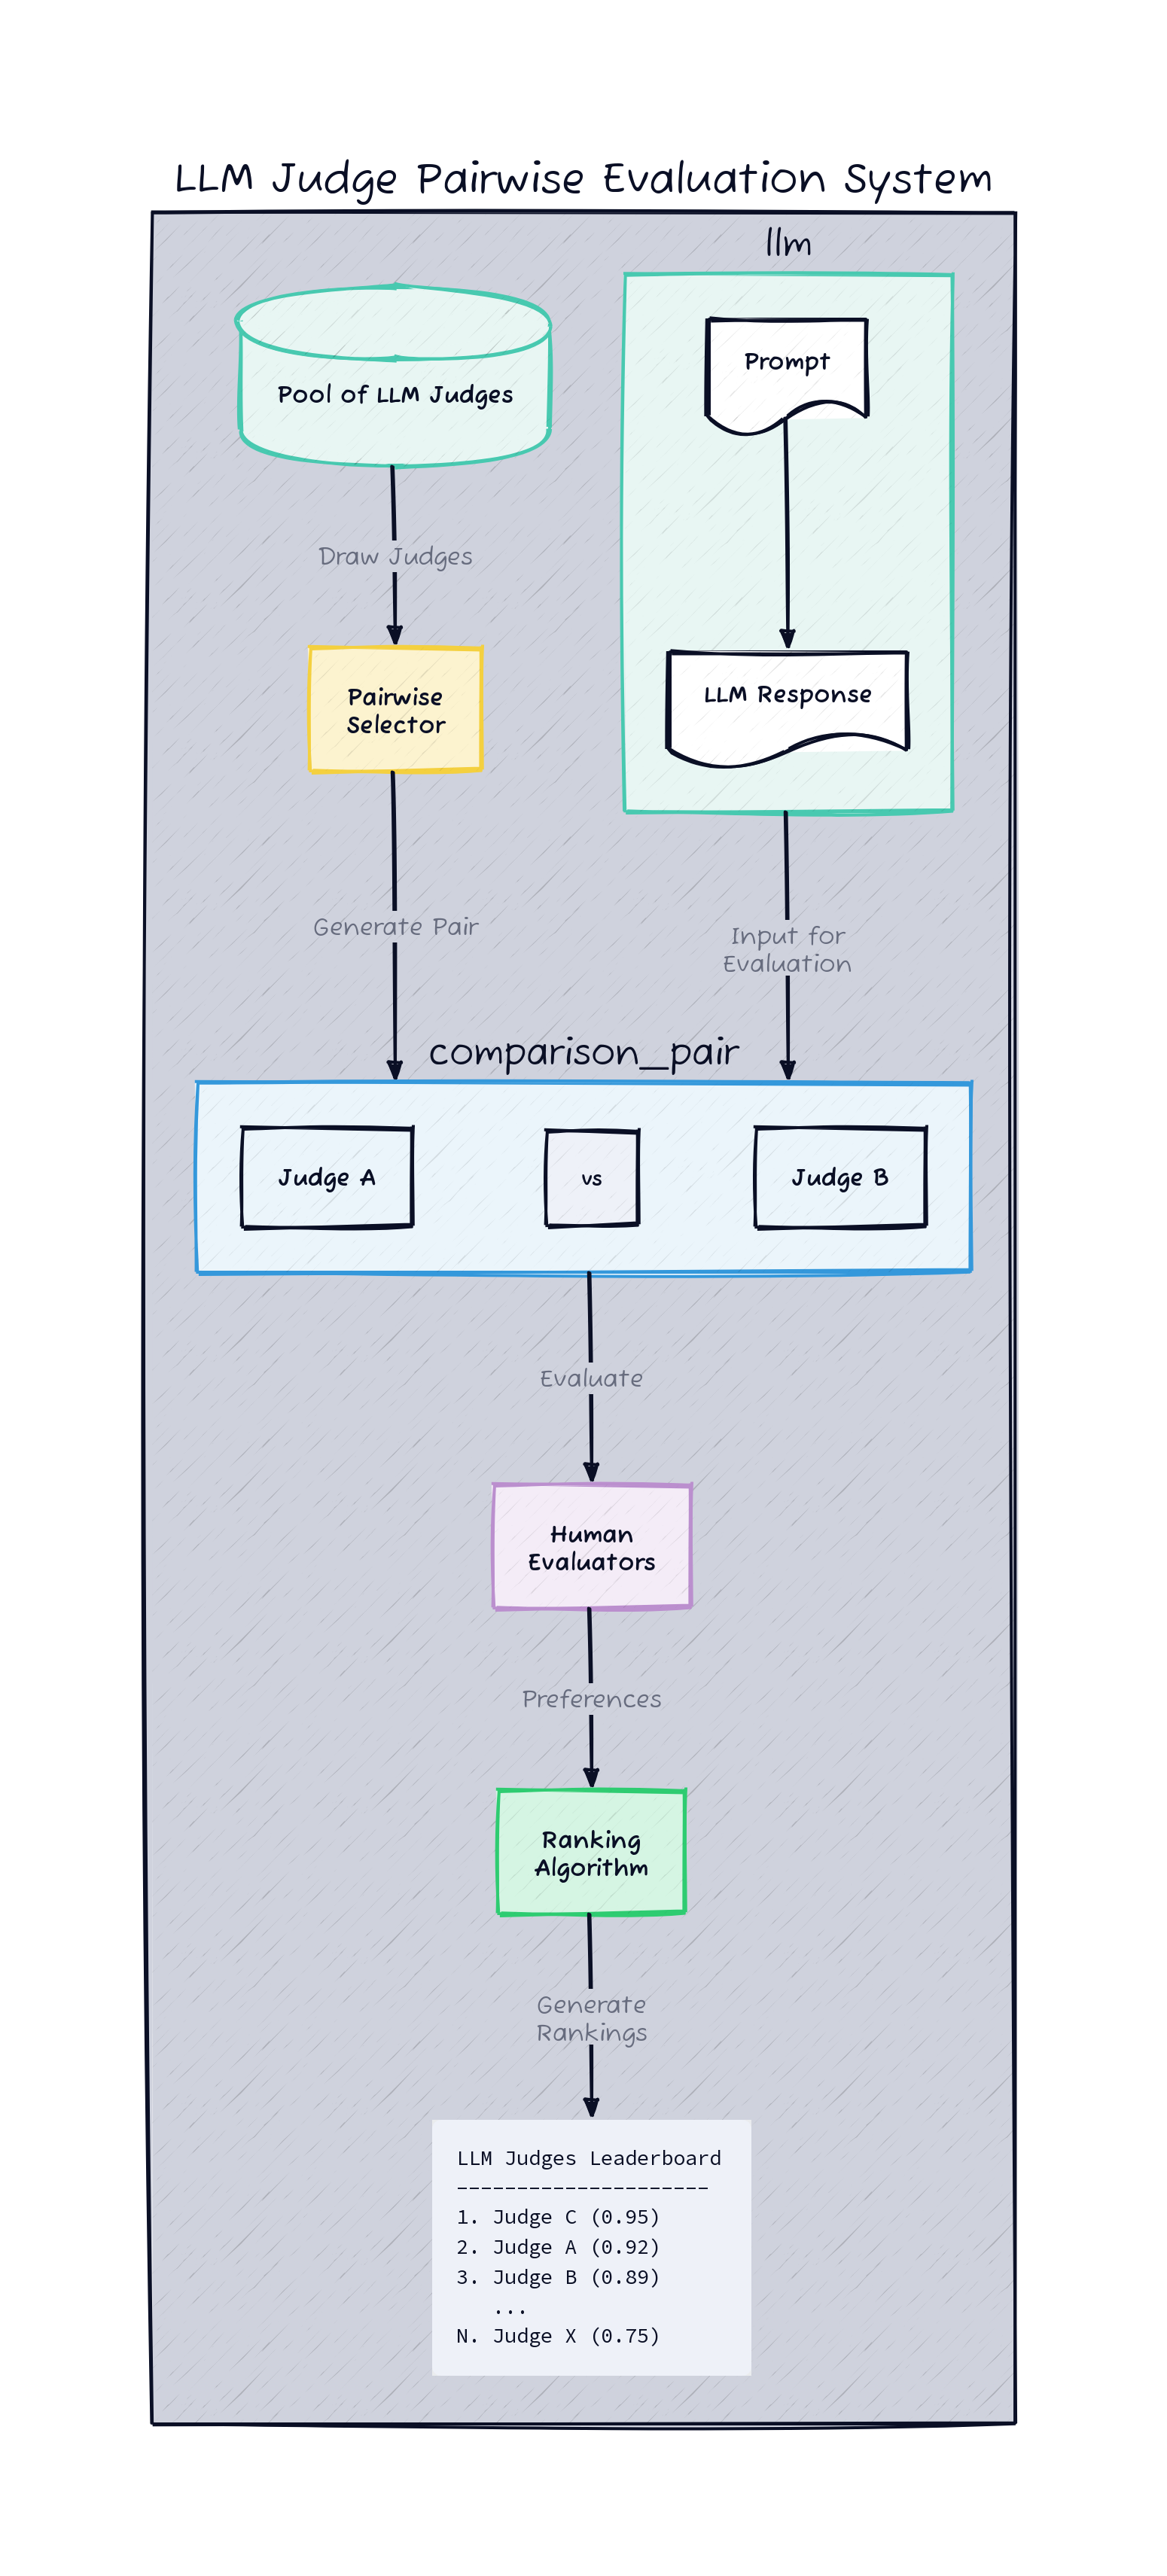
\includegraphics{evals/meta2.png}
\caption{Human-in-the-loop Meta Evaluation}
\label{fig:meta2}
\end{figure}

The LLM input and its prompt are displayed to the human evaluator and are customizable enabling task-specific meta evaluation. Further, the Judge Arena's LLM Judge's prompt is also editable by the user. Its default prompt is presented below:
\begin{quote}
Does the model provide relevant and useful responses to the user's needs or questions?

\textbf{Scoring Rubric:}

Score 1: The model's responses are irrelevant or unhelpful to the user's needs or queries.

Score 2: The model sometimes provides helpful information, but often fails to address the user's actual needs or questions.

Score 3: The model generally provides helpful responses that address the user's needs, though it may occasionally miss the mark.

Score 4: The model regularly provides helpful responses that are well-aligned with the user's inquiries, with only rare inaccuracies.

Score 5: The model consistently offers highly relevant and useful responses that perfectly cater to the user's needs and inquiries.
\end{quote}

Judge Arena's approach and policy framework has three key benefits worth highlighting:
\begin{enumerate}
    \item Transparency through open-source code, documentation, and data sharing
    \item LLM inclusion criteria requiring scoring/critique capabilities and public accessibility
    \item ELO-based leaderboard system with community involvement in evaluations
\end{enumerate}

In that way, the platform enables democratic evaluation of AI judges while maintaining transparency and accessibility standards.

\section{Benchmarks and Leaderboards}

Benchmarks act as standardized tests for LLMs, evaluating their performance across a spectrum of tasks. These tasks simulate real-world applications such as answering questions, generating coherent text, solving mathematical problems, or even writing computer code. They also assess more abstract qualities like fairness, robustness, and cultural understanding.

Benchmarks can be thought as comprehensive ``exams'' that probe different ``subjects'' in order to certify an LLM. They help researchers and developers compare models systematically, in a way LLM performance is comparable while enabling the identification of emergent behaviors or capabilities as models evolve in scale and sophistication.

The history of LLM benchmarks reflects the evolving priorities of artificial intelligence research, starting with foundational tasks and moving toward complex, real-world challenges. We can start in 2018 with the introduction of \textbf{GLUE} (General Language Understanding Evaluation) \sidecite{wang2019gluemultitaskbenchmarkanalysis}, which set a new standard for evaluating natural language understanding. GLUE measured performance on tasks like sentiment analysis and textual entailment, providing a baseline for assessing the fundamental capabilities of language models. Later, \textbf{SuperGLUE} \sidecite{nangia2019superglue} expanded on this foundation by introducing more nuanced tasks that tested reasoning and language comprehension at a deeper level, challenging the limits of models like BERT and its successors.

As AI capabilities grew, benchmarks evolved to capture broader and more diverse aspects of intelligence. \textbf{BIG-Bench} \sidecite{srivastava2023imitationgamequantifyingextrapolating} marked a turning point by incorporating over 200 tasks, spanning arithmetic, logic, and creative problem-solving. This collaborative effort aimed to probe emergent abilities in large models, offering insights into how scale and complexity influence performance. Around the same time, specialized benchmarks like \textbf{TruthfulQA} \sidecite{2021truthfulqa} emerged, addressing the critical need for models to provide accurate and non-deceptive information in a world increasingly dependent on AI for factual content.

\textbf{MMLU} (Massive Multitask Language Understanding) \sidecite{hendrycks2021measuringmassivemultitasklanguage} launched in 2021, provided a rigorous test of a model's multidisciplinary knowledge, covering 57 subjects from STEM fields to humanities and social sciences. Similarly, in 2022, Stanford's \textbf{HELM} (Holistic Evaluation of Language Models) \sidecite{liang2023holisticevaluationlanguagemodels} set a new standard for multidimensional assessment. HELM expanded the scope of evaluation beyond accuracy, incorporating factors like fairness, robustness, and computational efficiency. This benchmark was designed to address societal concerns surrounding AI, emphasizing safety and inclusion alongside technical performance. 

Specialized benchmarks like \textbf{HumanEval} (2021) \sidecite{chen2021evaluatinglargelanguagemodels} focused on domain-specific tasks, such as code generation, testing models' ability to translate natural language descriptions into functional programming code. In contrast, \textbf{LMSYS} (2023) brought real-world applicability into focus by evaluating conversational AI through multi-turn dialogues. LMSYS prioritized coherence, contextual understanding, and user satisfaction, providing a practical lens for assessing models like GPT and Claude in dynamic settings.

The \textbf{HuggingFace Open LLM} \sidecite{openllmleaderboard2024} Leaderboard stands out for its transparency and accessibility in the open-source community. This leaderboard evaluates a wide range of LLMs across diverse tasks, including general knowledge, reasoning, and code-writing. Its commitment to reproducibility ensures that results are verifiable, enabling researchers and practitioners to replicate findings. By focusing on open-source models, it democratizes AI research and fosters innovation across communities, making it a valuable resource for both academics and industry professionals.

The \textbf{Chatbot Arena} (2024) Leaderboard (an evolution of LMSYS) \sidecite{chiang2024chatbotarenaopenplatform} takes an alternative approach by measuring real-world performance through direct model comparisons. Its evaluation format compares models in live conversations, with human judges providing qualitative assessments. This methodology has gathered hundreds of thousands of human evaluations, offering specific insights into practical model performance. The emphasis on interactive capabilities makes it relevant for developing user-facing applications like virtual assistants and chatbots.

The \textbf{AlpacaEval} \sidecite{dubois2024lengthcontrolledalpacaevalsimpleway} and \textbf{MT-Bench} \sidecite{zheng2023judgingllmasajudgemtbenchchatbot} Leaderboards implement automated evaluation using LLMs to assess model performance in multi-turn conversations. This approach enables consistent assessment of dialogue capabilities while reducing human bias. Their methodology measures key aspects of conversational AI, including contextual understanding and response consistency across multiple exchanges.

An important recent development was the release of Global-MMLU \sidecite{singh2024globalmmluunderstandingaddressing}, an improved version of MMLU with evaluation coverage across 42 languages. This open dataset, built through collaboration between Argilla, the Hugging Face community, and researchers from leading institutions like Cohere For AI, Mila, MIT, and others, represents a significant step toward more inclusive multilingual LLM evaluation. Hundreds of contributors used Argilla to annotate MMLU questions, revealing that $85\%$ of questions requiring specific cultural knowledge were Western-centric. The newly released dataset is divided into two key subsets: Culturally Agnostic questions that require no specific regional or cultural knowledge, and Culturally Sensitive questions that depend on dialect, cultural, or geographic knowledge. With high-quality translations available for 25 languages, Global-MMLU enables better understanding of LLM capabilities and limitations across different languages and cultural contexts.

A major challenge with these leaderboards and benchmarks is test set contamination - when test data ends up in newer models' training sets, rendering the benchmarks ineffective. While some benchmarks try to address this through crowdsourced prompts and evaluations from humans or LLMs, these approaches introduce their own biases and struggle with difficult questions. \textbf{LiveBench} \sidecite{white2024livebenchchallengingcontaminationfreellm} represents a novel solution, designed specifically to be resilient to both contamination and evaluation biases. As the first benchmark with continuously updated questions from recent sources, automated objective scoring, and diverse challenging tasks across multiple domains, LiveBench maintains its effectiveness even as models improve. Drawing from recent math competitions, research papers, news, and datasets, it creates contamination-free versions of established benchmark tasks. Current results show even top models achieving considerably lower performance compared to other benchmarks, demonstrating LiveBench's ability to meaningfully differentiate model capabilities with relatively lower saturation. With monthly updates and an open collaborative approach, LiveBench aims to provide sustained value for model evaluation as the field advances.

Another notable benchmark is ZebraLogic \sidecite{zebralogic2024}, which evaluates logical reasoning capabilities of LLMs through Logic Grid Puzzles - a type of Constraint Satisfaction Problem \sidecite{brailsford1999constraint} commonly found in tests like the LSAT. These puzzles require assigning unique values to $N$ houses across $M$ different features based on given clues, demanding strategic reasoning and deduction to arrive at a unique correct solution. The benchmark's programmatically generated puzzles range from $2\times2$ to $6\times6$ in size and test LLMs using one-shot examples with reasoning steps. While humans can solve these puzzles through strategic methods like reductio ad absurdum and elimination, LLMs demonstrate significant limitations in this type of logical reasoning. Even the best-performing model, Claude 3.5 Sonnet, only achieves $33.4\%$ accuracy across all puzzles and $12.4\%$ on hard puzzles, with smaller models (7-10B parameters) solving less than $1\%$ of hard puzzles as of December 2024. These results reveal critical gaps in LLMs' capabilities around counterfactual thinking, reflective reasoning, structured memorization, and compositional generalization.

A significant milestone in AI evaluation came with the launch of the \textbf{The Alignment Research Center (ARC) Prize} \sidecite{arcprize2024} by ARC Prize Inc., a non-profit for the public advancement of open artificial general intelligence. Hosted by Mike Knoop (Co-founder, Zapier) and François Chollet (Creator of Keras), this prize represents a paradigm shift in how we evaluate language models. Rather than focusing on narrow performance metrics, the ARC Prize assesses what it calls ``cognitive sufficiency'' - a model's ability to generate meaningful insights and tackle open-ended challenges. This new way to think about LLM evaluation emphasizes creative thinking, sophisticated reasoning, and the capacity to make genuinely useful contributions to human knowledge. Arguably, it is an attempt to define and measure a step towards what it means to achieve AGI (Artificial General Intelligence).

\begin{quote}
\textbf{Defining AGI according to ARC Prize:}

Consensus but wrong:
\begin{itemize}
    \item AGI is a system that can automate the majority of economically valuable work.
\end{itemize}

Correct:
\begin{itemize}
    \item AGI is a system that can efficiently acquire new skills and solve open-ended problems.
\end{itemize}
\end{quote}

The ARC benchmark distinguishes itself from other LLM benchmarks especially in its resistance to memorization by prioritizing:

\begin{itemize}
    \item \textbf{Focus on Core Knowledge:} Unlike LLM benchmarks that test a broad range of knowledge and skills, often relying heavily on memorization, ARC focuses on core knowledge similar to what a four or five-year-old child might possess. This includes basic concepts like object recognition, counting, and elementary physics.

    \item \textbf{Novelty of Tasks:} Each ARC puzzle is designed to be novel, meaning it's something you likely wouldn't have encountered before, even if you had memorized the entire internet. This characteristic directly challenges the way LLMs typically operate, which is by leveraging their vast ``interpolative memory.''

    \item \textbf{Emphasis on Program Synthesis:} ARC tasks require models to synthesize new solution programs on the fly for each unique puzzle. This stands in contrast to the more common LLM approach of retrieving pre-existing solution programs from memory.

    \item \textbf{Resistance to Brute Force Attempts:} While acknowledging the possibility, ARC aims to be resistant to brute-force approaches where a model might be trained on millions of similar puzzles to achieve a high score by relying on overlap with the test set.
\end{itemize}

ARC-AGI tasks are a series of three to five input and output tasks followed by a final task with only the input listed (e.g. Figure~\ref{arc}). Each task tests the utilization of a specific learned skill based on a minimal number of cognitive priors. A successful submission is a pixel-perfect description (color and position) of the final task's output.

\begin{figure}[h]
\centering
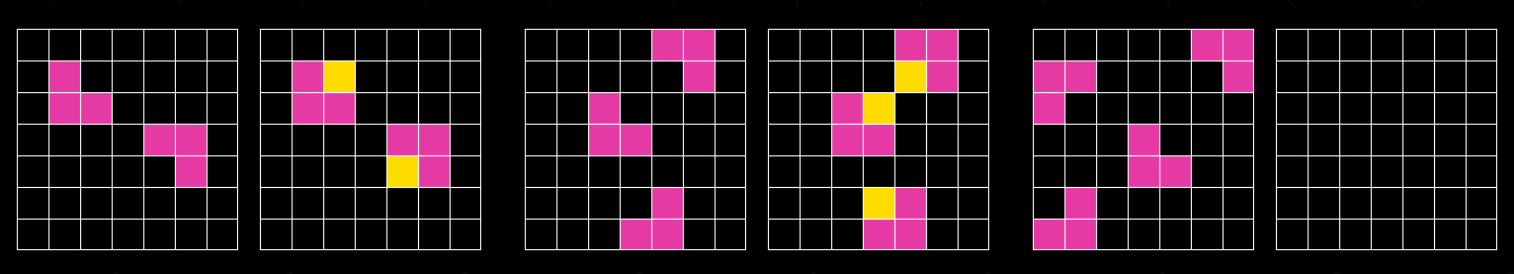
\includegraphics[scale=0.5]{evals/arc.png}
\label{arc}
\end{figure}
These features make the ARC benchmark a unique test of machine intelligence, focusing on the ability to adapt to novelty and solve problems without relying heavily on memorization. This is more aligned with the concept of general intelligence, which emphasizes the ability to learn efficiently and tackle new challenges.

The ARC-AGI benchmark remained unbeaten for five years as of December 2024 (a minimum score of $85\%$ in the private dataset is required to win) \sidecite{arcprizeresults2024}. A key takeaway is that algorithmic improvements, rather than massive computational resources, may be key to exceeding the target score for the ARC-AGI benchmark.

In addition to the benchmarks discussed above, a growing set of domain-specific benchmarks is emerging to help evaluate LLMs in specific verticals, including:
\begin{itemize}
    \item \textbf{FinBench} \sidecite{zhang2024finbench}: Evaluates LLMs in the financial domain, covering tasks such as terminology understanding, temporal reasoning, future forecasting, scenario planning, and numerical modelling.
    \item \textbf{LegalBench} \sidecite{guha2023legalbench}: Assesses the legal reasoning abilities of LLMs through tasks crowdsourced by legal professionals
    \item \textbf{Berkeley Function Leaderboard (BFCL)} \sidecite{patil2023gorilla}: Evaluates LLMs' function-calling abilities
\end{itemize}

As language models continue to advance in capability and complexity, evaluation frameworks must evolve. Modern benchmarks increasingly incorporate tests for nuanced reasoning, ethical decision-making, and emergent capabilities that weren't previously measurable. This ongoing evolution reflects a deeper understanding that the true value of language models lies not in achieving high scores on standardized tests with narrow task-specific metrics, but in their ability to meaningfully contribute to human understanding and help solve real-world problems while demonstrating the ability to learn and adapt to new tasks.

In the following sections, we will explore some open source tools developers can use to automate and streamline the challenging task of LLMs evals.
\section{Tools}

\subsection{LightEval}

LightEval \sidecite{lighteval} is a lightweight framework for evaluation of LLMs across a variety of standard and bespoke metrics and tasks across multiple inference backends via Python SDK and CLI.

As a motivating example, consider a scenario where financial data has been extracted from SEC financial filings and require econometric analysis. Tasks like estimating autoregressive models for time series forecasting or conducting hypothesis tests on market efficiency are common in financial analysis. Let's evaluate how well different models perform on this type of task.

First, we need to select a benchmark to assess LLMs capabilities in this domain. MMLU has a sub-benchmark called Econometrics we can use for this task. Table~\ref{mmlu-econometrics} shows a sample of the benchmark dataset from MMLU Econometrics. It consists of multiple-choice questions from econometrics and expected answers.

\begin{table*}[h]
\caption{MMLU Econometrics Task Dataset sample}
\label{mmlu-econometrics}
\begin{tabular}{p{0.3\textwidth}p{0.3\textwidth}p{0.15\textwidth}p{0.1\textwidth}p{0.15\textwidth}}
\hline
Question & Options & Correct Options & Index & Literal \\
\hline
Consider the following AR(1) model with the disturbances having zero mean and unit variance: $y_t = 0.2 + 0.4 y_{t-1} + u_t$ The (unconditional) mean of y will be given by & ["0.2", "0.4", "0.5", "0.33"] & ["b"] & [3] & ["0.33"] \\
\hline
Suppose that a test statistic has associated with it a p-value of 0.08. Which one of the following statements is true? (i) If the size of the test were exactly 8\%, we... & ["(ii) and (iv) only", "(i) and (iii) only", "(i), (ii), and (iii) only", "(i), (ii), (iii), and (iv)"] & ["c"] & [2] & ["(i), (ii), and (iii) only"] \\
\hline
What would be then consequences for the OLS estimator if heteroscedasticity is present in a regression model but ignored? & ["It will be biased", "It will be inconsistent", "It will be inefficient", "All of (a), (b) and (c) will be true."] & ["c"] & [2] & ["It will be inefficient"] \\
\hline
Suppose now that a researcher wishes to use information criteria to determine the optimal lag length for a VAR. 500 observations are available for the bivariate VAR... & ["1 lag", "2 lags", "3 lags", "4 lags"] & ["c"] & [2] & ["3 lags"] \\
\hline
\end{tabular}
\end{table*}
The code sample below demonstrates the LightEval Python SDK framework for evaluating a target LLM model on a given task. First, we instantiate an \texttt{EvaluationTracker} which manages result storage, in this example kept in a local directory \texttt{output\_dir}, and tracks detailed evaluation metrics, optionally pushed to HuggingFace Hub.

Next, we instantiate an object of the class \texttt{PipelineParameters} which, in this example, configures the pipeline for parallel processing with a temporary cache in \texttt{cache\_dir} also setting the maximum number of samples to process to \texttt{max\_samples}. Then, in \texttt{BaseModelConfig} we set up the LLM model we would like to evaluate defined in \texttt{pretrained}.

\begin{minted}{bash}
pip install lighteval[accelerate]
\end{minted}
\begin{minted}{python}
import lighteval
from lighteval.logging.evaluation_tracker import EvaluationTracker
from lighteval.models.model_config import BaseModelConfig
from lighteval.pipeline import ParallelismManager, Pipeline, PipelineParameters
from lighteval.utils.utils import EnvConfig
from lighteval.utils.imports import is_accelerate_available
from datetime import timedelta
from accelerate import Accelerator, InitProcessGroupKwargs


def create_evaluation_pipeline(output_dir: str, cache_dir: str, pretrained: str, dtype: str = "float16", max_samples: int = 10, task: str):
    if is_accelerate_available():
        from accelerate import Accelerator, InitProcessGroupKwargs
        accelerator = Accelerator(kwargs_handlers=[InitProcessGroupKwargs(timeout=timedelta(seconds=3000))])
    else:
        accelerator = None

    evaluation_tracker = EvaluationTracker(
        output_dir=output_dir,
        save_details=True,
        push_to_hub=False  
    )

    pipeline_params = PipelineParameters(
        launcher_type=ParallelismManager.ACCELERATE,
        env_config=EnvConfig(cache_dir=cache_dir),
        override_batch_size=1,
        max_samples=max_samples
    )

    model_config = BaseModelConfig(
        pretrained=pretrained,
        dtype=dtype,
        use_chat_template=True,
        trust_remote_code=True
    )

    pipeline = Pipeline(
        tasks=task,
        pipeline_parameters=pipeline_params,
        evaluation_tracker=evaluation_tracker,
        model_config=model_config
    )
    
    return pipeline
\end{minted}
Figure~\ref{fig:lighteval} shows a schematic representation of its key components. As inference engine, we leverage \texttt{accelerate} for distributed evaluation. \texttt{lighteval} also supports other inference backends such as \texttt{vllm} and \texttt{tgi}.

\begin{figure}[h]
\centering
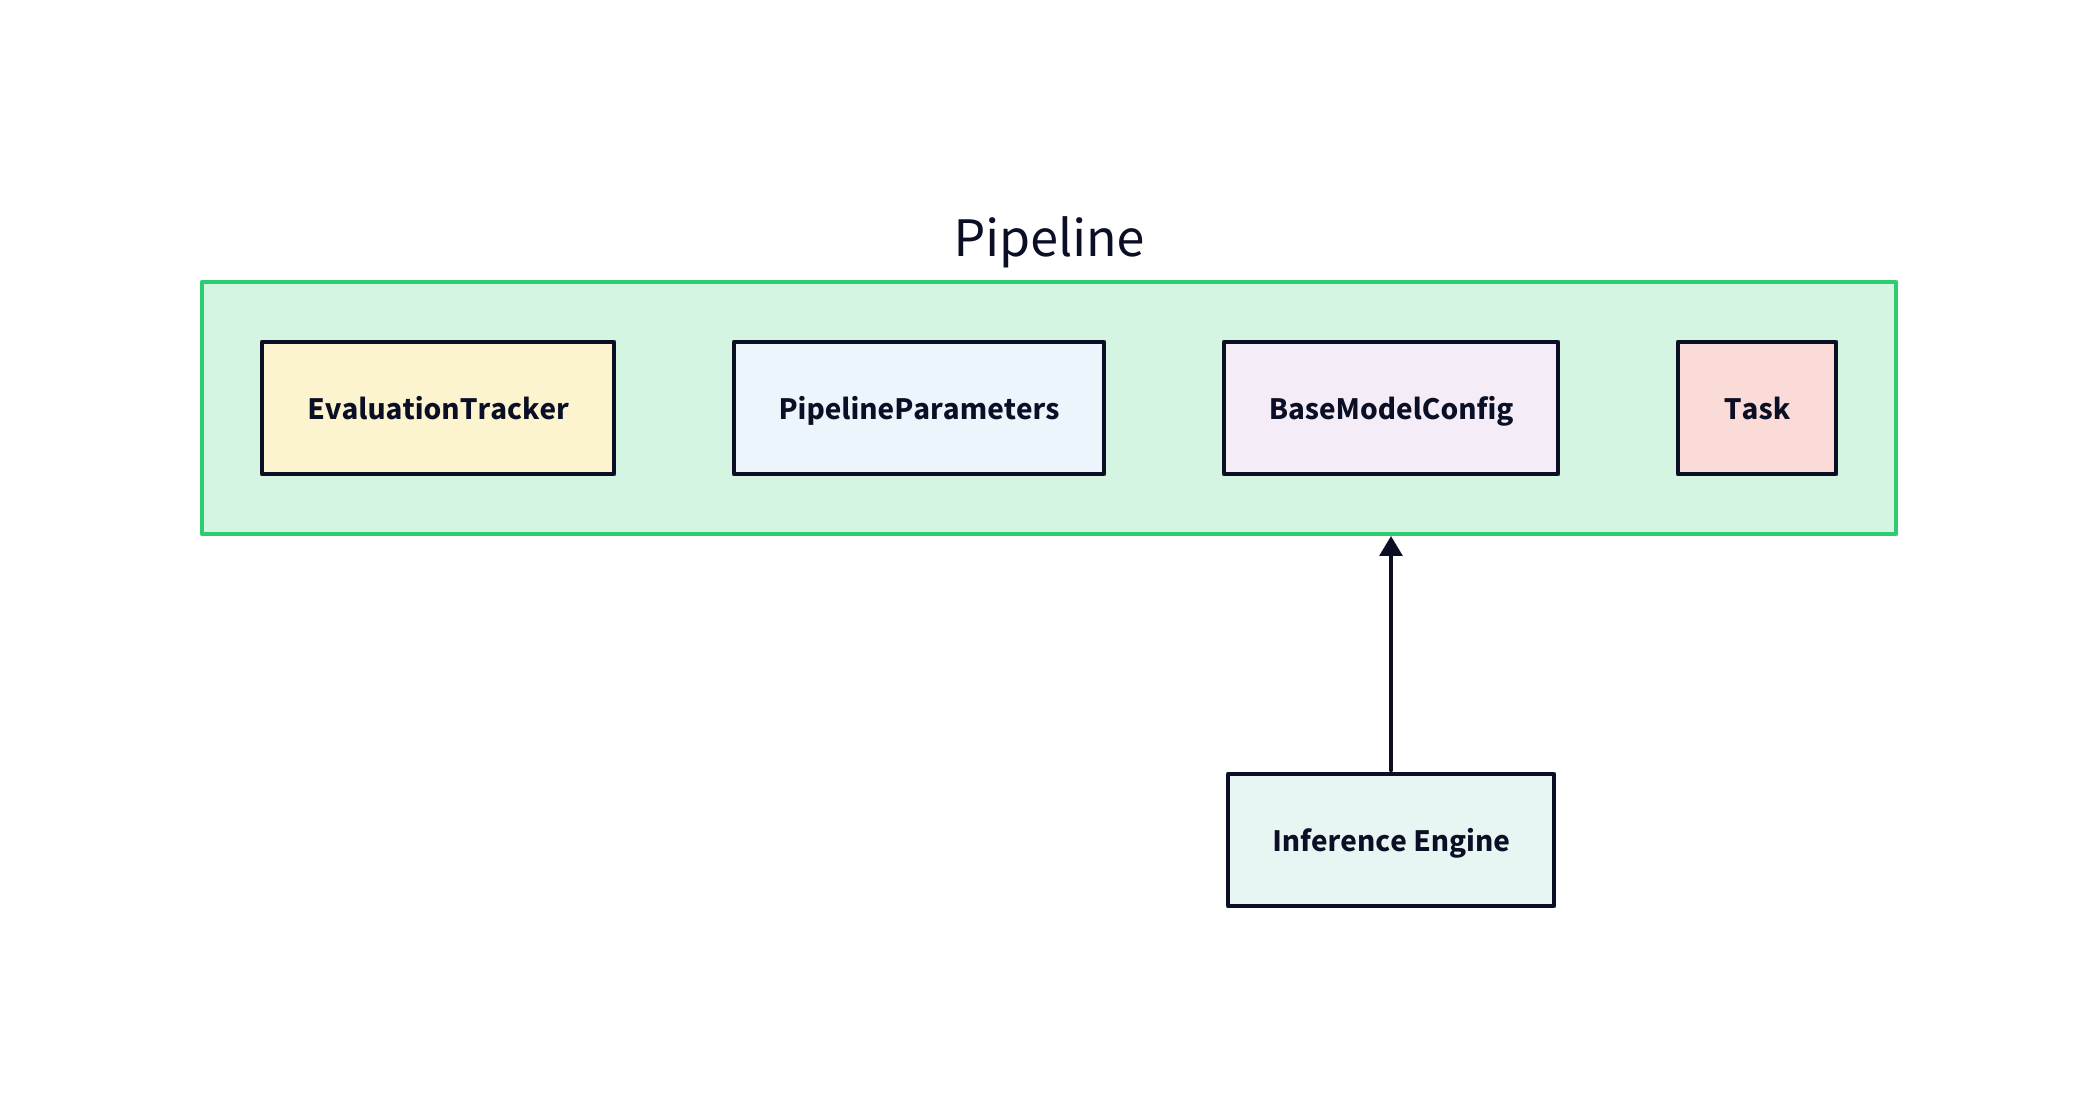
\includegraphics{evals/lighteval.png}
\caption{LightEval Python SDK Sample Conceptual Overview.}
\label{fig:lighteval}
\end{figure}

This setup allows for systematic evaluation of language model performance on specific tasks while handling distributed computation and result tracking.

The final Pipeline combines these components to evaluate in the user defined \texttt{task}, which follows the following format:

\begin{minted}{bash}
\{suite\}|\{task\}|\{num_few_shot\}|\{0 or 1 to automatically reduce num_few_shot if prompt is too long\}
\end{minted}

The task string format follows a specific pattern with four components separated by vertical bars ($|$):

\begin{enumerate}
\item suite: The evaluation suite name (e.g., ``leaderboard'')
\item task: The specific task name (e.g., ``mmlu:econometrics'') 
\item num\_few\_shot: The number of few-shot examples to use (e.g., ``0'' for zero-shot)
\item A binary flag (0 or 1) that controls whether to automatically reduce the number of few-shot examples if the prompt becomes too long
\end{enumerate}
LightEval provides a comprehensive set of evaluation tasks \sidecite{lighteval_tasks} and metrics \sidecite{lighteval_metrics}. The available tasks span multiple categories and benchmarks including BigBench, MMLU, TruthfulQA, WinoGrande, and HellaSwag. The framework also supports standard NLP evaluation metrics including BLEU, ROUGE, Exact Match, F1 Score, and Accuracy.

In our case, we choose to evaluate our LLMs on the MMLU econometrics task using zero-shot learning. Hence, we define the \texttt{task} as follows:

\begin{minted}{python}
task = "leaderboard|mmlu:econometrics|0|0"
\end{minted}

Example usage to evaluate an LLM, for instance \texttt{meta-llama/Llama-3.2-1B-Instruct}, on the MMLU econometrics task using zero-shot learning:

\begin{minted}{python}
task = "leaderboard|mmlu:econometrics|0|0"
model = "meta-llama/Llama-3.2-1B-Instruct"
pipeline = create_evaluation_pipeline(output_dir="./evals/", 
                                   cache_dir="./cache/", 
                                   pretrained=model, 
                                   task=task)
\end{minted}
We can then evaluate the pipeline, save and show its results as follows:

\begin{minted}{python}
pipeline.evaluate()
pipeline.save_and_push_results()
pipeline.show_results()
\end{minted}

The results are then stored in \texttt{output\_dir} in JSON format.

The same results can be obtained by using the LightEval CLI:

\begin{minted}{bash}
lighteval accelerate --model_args "pretrained=meta-llama/Llama-3.2-1B-Instruct" --tasks "leaderboard|mmlu:econometrics|0|0" --override_batch_size 1 --output_dir="./evals/"
\end{minted}
Comparing the performance of multiple open source models on the MMLU econometrics task requires careful consideration of computational resources. While local evaluation is possible, leveraging a remote server proves more efficient in terms of time and resources. LightEval facilitates this by enabling model serving on a TGI-compatible server/container and executing evaluations through server requests \sidecite{lighteval_server}.

The HuggingFace Serverless Inference API provides an ideal solution for this purpose\sidenote{A bug was discovered in LightEval that initially prevented compatibility with the HuggingFace Serverless Inference API: \url{https://github.com/huggingface/lighteval/issues/422}. The LightEval team has since resolved this issue.}. The configuration file for LightEval should be structured as follows, where \texttt{<MODEL-ID>} represents the model identifier on HuggingFace (e.g., \texttt{meta-llama/Llama-3.2-1B-Instruct}) and \texttt{<HUGGINGFACE-TOKEN>} is the user's HuggingFace API token. Alternatively, a URL for a dedicated inference API can be specified if available.

\begin{minted}{yaml}
model:
  type: "tgi"
  instance:
    inference_server_address: "https://api-inference.huggingface.co/models/<MODEL-ID>"
    inference_server_auth: "<HUGGINGFACE-TOKEN>"
    model_id: null
\end{minted}
Now we can run the evaluation by sending requests to the server as follows by using the same bash command as before but now setting the \texttt{model\_config\_path} to the path of the configuration file we have just created (e.g. \texttt{endpoint\_model.yaml}):

\begin{minted}{bash}
lighteval accelerate --model_config_path="endpoint_model.yaml" --tasks "leaderboard|mmlu:econometrics|0|0" --override_batch_size 1 --output_dir="./evals/"
\end{minted}

To complete our task, we evaluate a few models from the following model families: \texttt{Llama3.2}, \texttt{Qwen2.5}, and \texttt{SmolLM2} as described in Table~\ref{tab:model-families}.

\begin{table}[h]
\caption{Model Families Evaluated Using LightEval}
\label{tab:model-families}
\begin{tabular}{llll}
\hline
Model Family & Description & Models & References \\
\hline
Llama3.2 Instruct & LLaMA architecture-based pretrained & \texttt{Llama-3.2-1B-Instruct} & \sidecite{meta_llama_models} \\
 & and instruction-tuned generative models & \texttt{Llama-3.2-3B-Instruct} & \\
\hline
Qwen2.5 Instruct & Instruction-tuned LLMs family & \texttt{Qwen2.5-0.5B-Instruct} & \sidecite{gpt2docs,hui2024qwen2,qwen2} \\
 & built by Alibaba Cloud & \texttt{Qwen2.5-1.5B-Instruct} & \\
 & & \texttt{Qwen2.5-3B-Instruct} & \\
\hline
SmolLM2 Instruct & Instruction-tuned family of compact & \texttt{SmolLM2-360M-Instruct} & \sidecite{allal2024SmolLM2} \\
 & language models built by HuggingFace & \texttt{SmolLM2-1.7B-Instruct} & \\
\hline
\end{tabular}
\end{table}
We can then compare the performance of these models on the MMLU econometrics task as shown in Figure~\ref{fig:model-comparison}.

\begin{figure}[h]
\centering
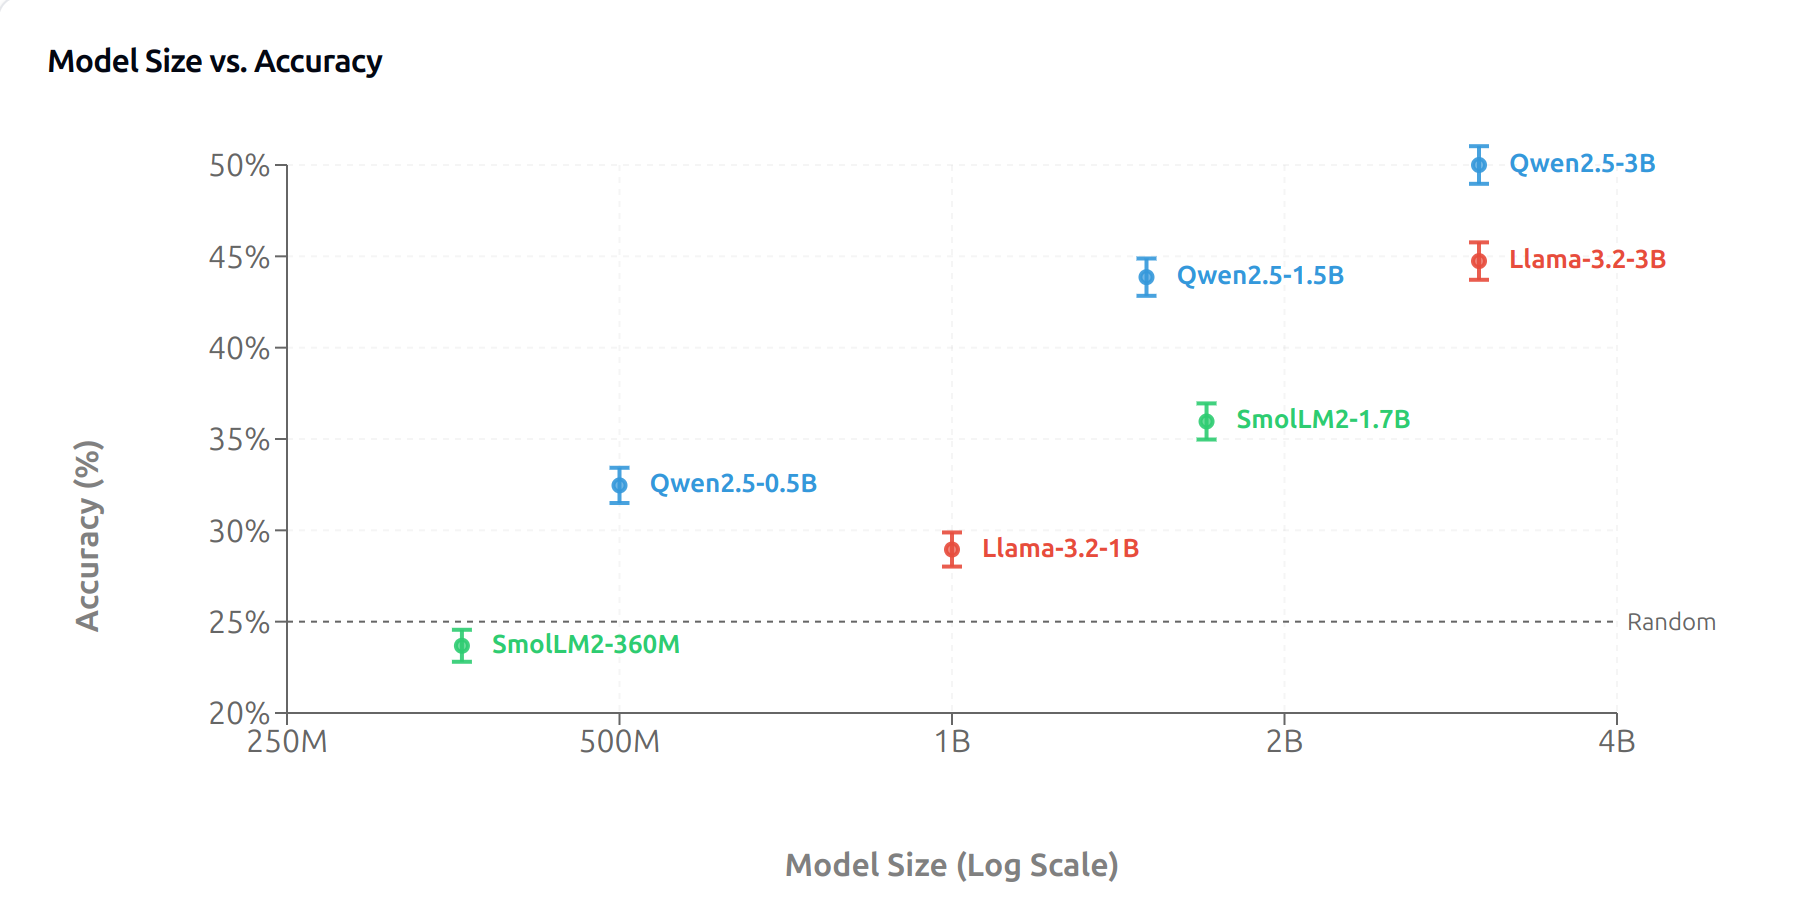
\includegraphics{evals/model-comparison.png}
\caption{Model performance comparison on MMLU Econometrics task, showing accuracy scores across different model sizes and architectures.}
\label{fig:model-comparison}
\end{figure}

The results reveal several interesting patterns in model performance. As expected, we observe a trend where larger models consistently achieve higher accuracy scores. The evaluation shows distinct clusters among model families, with Qwen2.5, Llama-3.2, and SmolLM2 each exhibiting their own scaling characteristics, suggesting that architectural differences lead to varying degrees of efficiency as model size increases. Particularly noteworthy is the performance of the Qwen2.5 family, which demonstrates superior accuracy even at smaller model sizes when compared to Llama-3.2.

Of course, the results should be taken with a grain of salt given the limited size of the dataset (MMLU Econometrics $\sim$ 100), limited number of models and sizes. However, it gives a good indication of the capabilities of the different models tested with Qwen2.5 family being an interesting first candidate as a relatively small yet powerful model demonstrating a good trade-off between performance and size. Once tested on real-world data, the results will change but these initial findings are a good data-driven starting point for model selection as you begin your LLM-based application development.

In summary, LightEval is a simple yet flexible and comprehensive framework for evaluating LLMs across a wide variety of tasks and metrics. It can serve as a first step in selecting your next LLM for a specific task given the exponential growth in number of (open source) models available \sidecite{hf_num_models}. Its integration with the Hugging Face ecosystem and modular architecture make it particularly powerful for evaluating open source models. For further details, visit the official repository\sidenote{\url{https://github.com/huggingface/lighteval}} \sidecite{lighteval}.
\subsection{LangSmith}

Let's revisit our evaluation example when we were interested in evaluating the quality of summaries generated by different (smaller and cheaper) LLM models compared to a benchmark model (larger and more expensive). Recall the setup:

\begin{itemize}
\item Benchmark model: \texttt{gpt-4o}
\item Test models: \texttt{gpt-4o-mini}, \texttt{gpt-4-turbo}, \texttt{gpt-3.5-turbo}
\end{itemize}

We can run evaluation using only LangSmith without the need of LangChain.

\begin{minted}{bash}
!pip uninstall langchain
!pip uninstall langchain-community 
!pip uninstall langchain-openai
!pip install langsmith
\end{minted}

We need to generate an API key to use LangSmith. See instructions at \url{https://docs.smith.langchain.com/}. Remember to export your API\_KEY. Activating tracing will allow us to track logs and foster observability of our evaluation.

\begin{minted}{bash}
export LANGCHAIN_TRACING_V2=true
export LANGCHAIN_API_KEY=<your-api-key>
\end{minted}

\begin{minted}{python}
import evaluate as hf_evaluate  # HuggingFace's evaluate
from langsmith import evaluate as langsmith_evaluate  # LangSmith's evaluate
from langsmith import Client
from typing import Dict, Any

ls_client = Client()
\end{minted}

The code below creates a dataset in LangSmith that will serve as our golden dataset for evaluation. The dataset consists of test cases where we create a single example with the following content:

\begin{itemize}
\item An input: Our SEC filing document
\item An expected output: A golden summary generated by our benchmark model (\texttt{gpt-4o})
\end{itemize}

This dataset will allow us to evaluate how well other models perform compared to our benchmark by comparing their generated summaries against these reference summaries. In practice, it's recommended to create a larger dataset with more diverse examples to get a more accurate assessment of model capabilities as well as to estimate confidence intervals for target metrics.

\begin{minted}{python}
# Define dataset: these are your test cases
dataset_name = "Golden SEC Summary Dataset"
dataset = ls_client.create_dataset(dataset_name)
ls_client.create_examples(
    inputs=[
        {"sec_filing": sec_filing},
    ],
    outputs=[
        {"summary": benchmark_summary},
    ],
    dataset_id=dataset.id,
)
\end{minted}
Our Dataset is now available in LangSmith as shown in Figure~\ref{fig:langsmith_dataset}.
\begin{figure}[h]
\centering
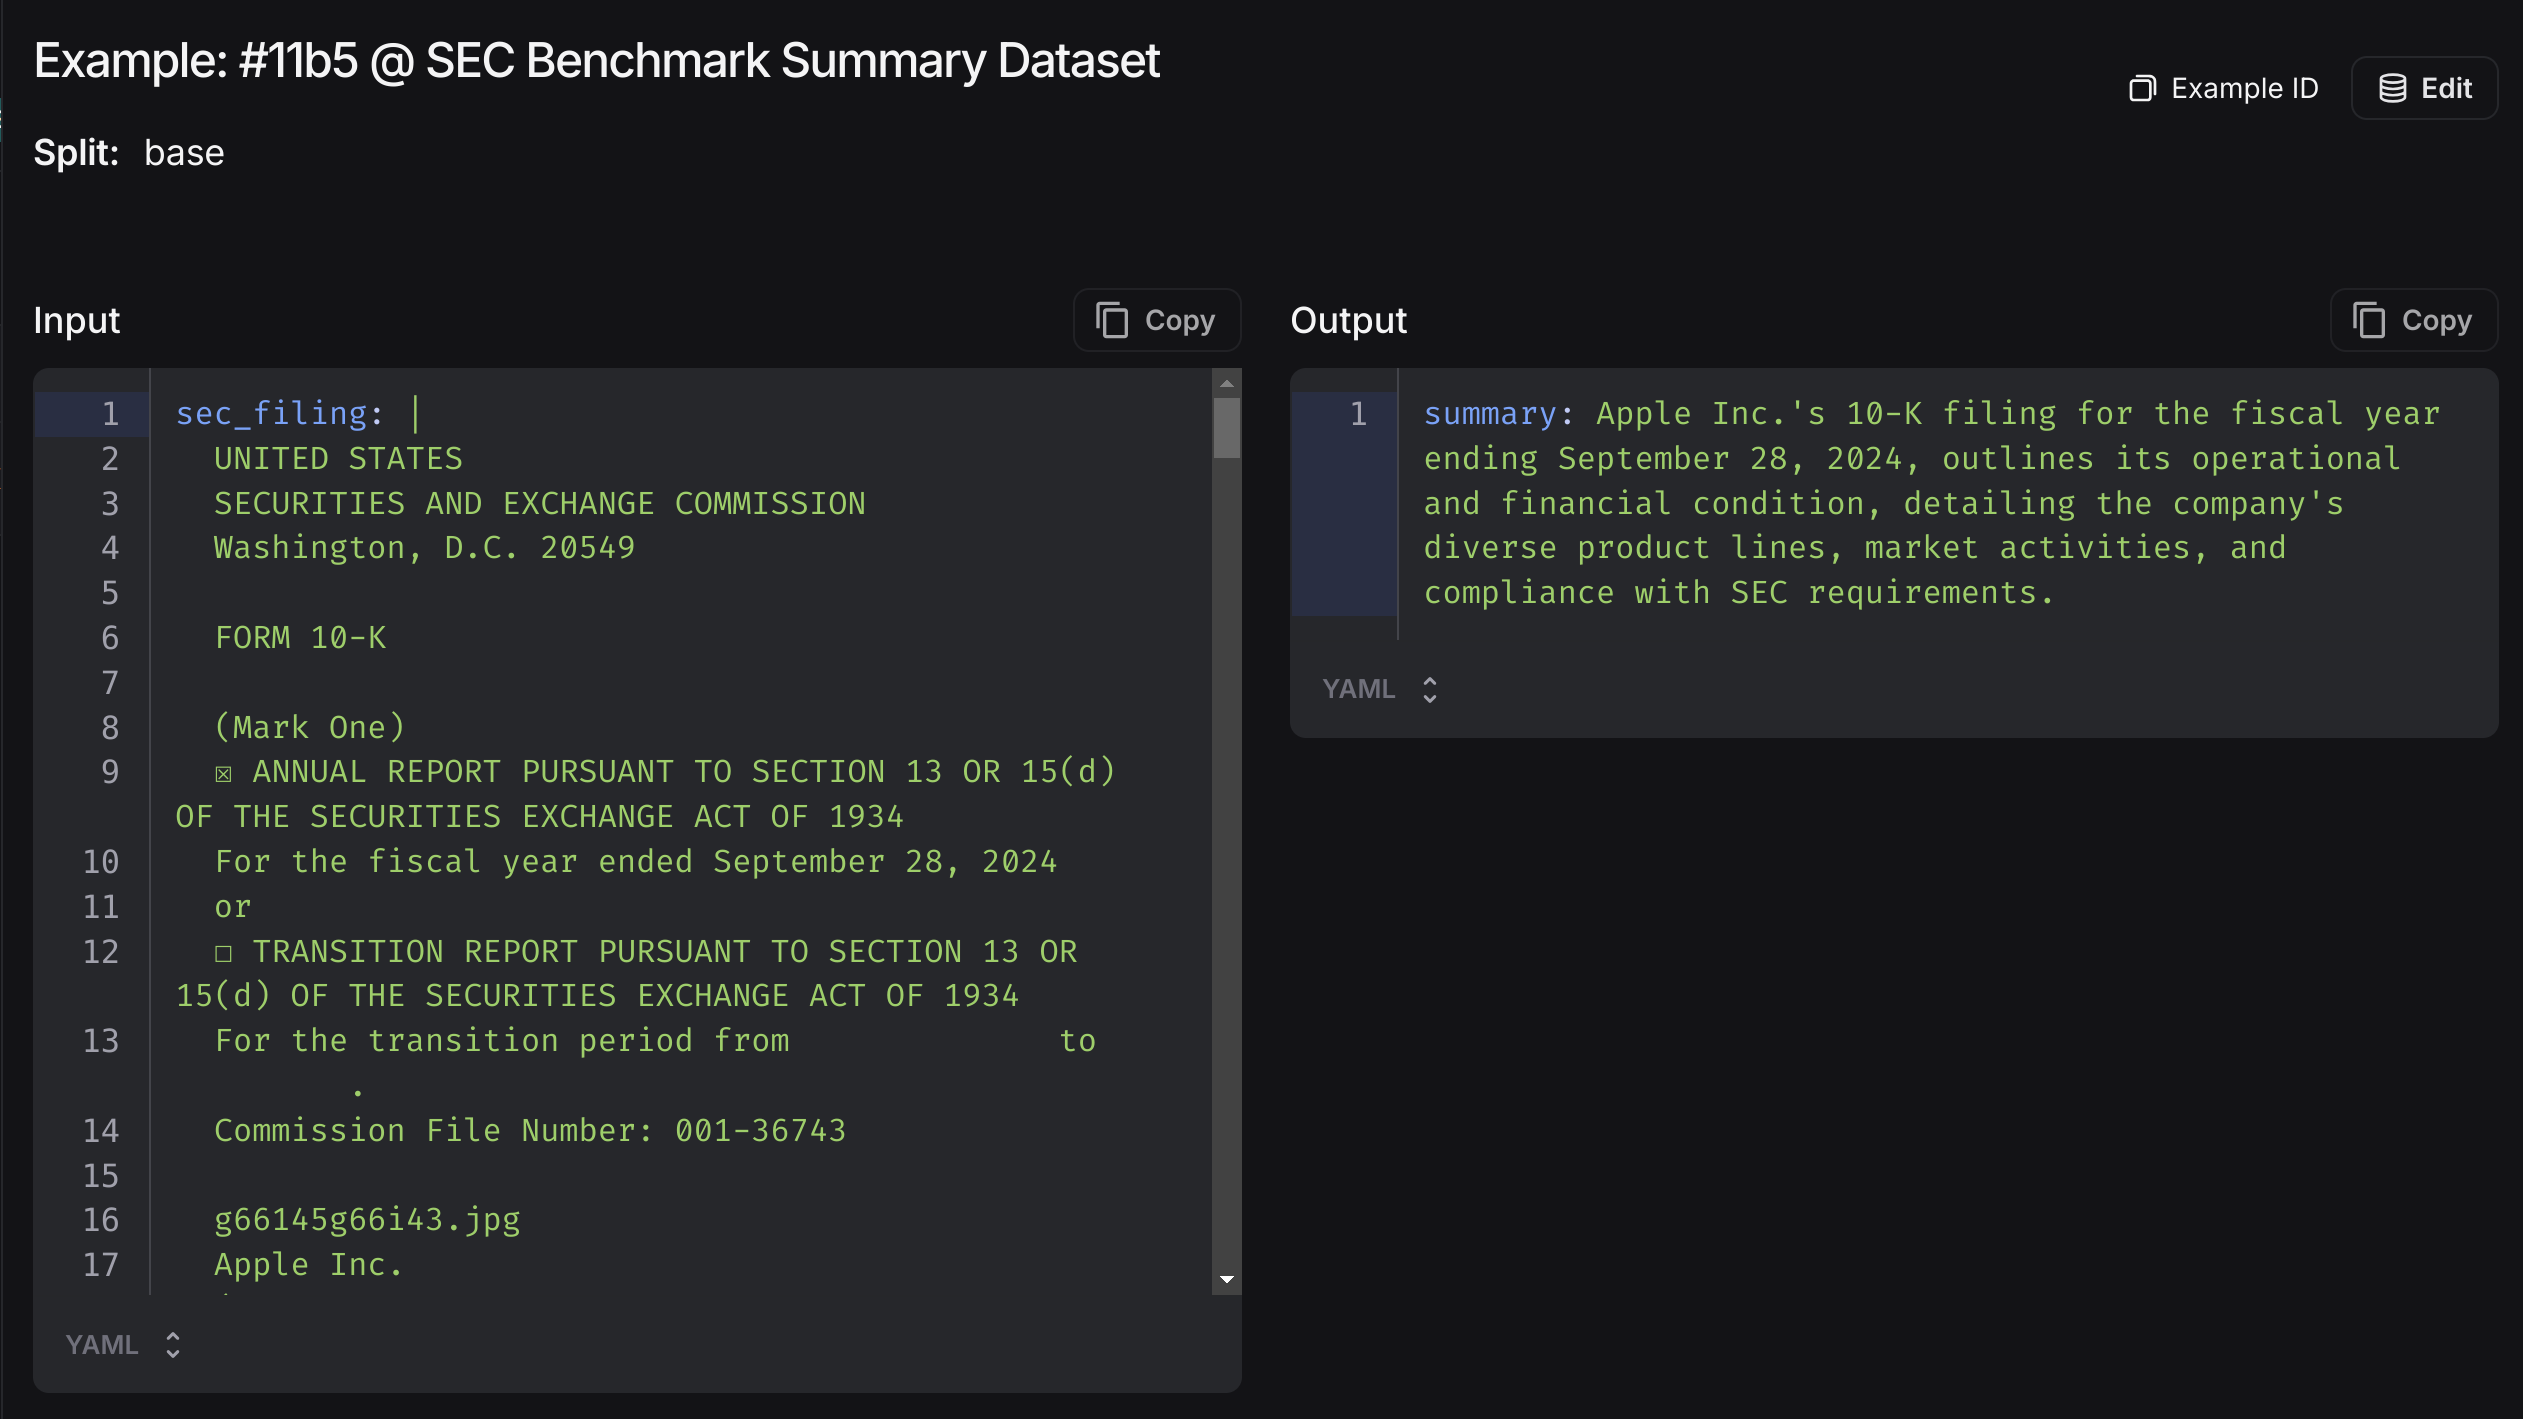
\includegraphics{evals/langsmith_dataset.png}
\label{fig:langsmith_dataset}
\caption{LangSmith Dataset}
\end{figure}

Next, we write our evaluator. This evaluator calculates BLEU scores between generated and reference summaries using HuggingFace's evaluate package. The evaluator takes two dictionaries as input - one containing the generated summary and another containing the reference summary. It returns a dictionary with the Google BLEU score, which measures the overlap between n-grams in the generated and reference texts similar to our previous metric-based experiments.

\begin{minted}{python}
def calculate_scores(outputs: Dict[str, Any], reference_outputs: Dict[str, Any]) -> dict:
    """
    Custom evaluator that calculates BLEU and ROUGE scores between generated and reference summaries
    using HuggingFace's evaluate package
    
    Args:
        outputs (dict): Contains the generated summary
        reference_outputs (dict): Contains the reference summary
    
    Returns:
        dict: Dictionary containing Google BLEU score
    """
    generated = outputs.get("summary", "")
    reference = reference_outputs.get("summary", "")
    
    # Initialize metrics from HuggingFace's evaluate
    bleu = hf_evaluate.load("google_bleu")
    
    # Format inputs for BLEU (expects list of str for predictions and list of list of str for references)
    predictions = [generated]
    references = [reference]
    
    # Compute BLEU score
    bleu_score = bleu.compute(predictions=predictions, references=[references])
    
    return {"key": "google_bleu", "score": bleu_score["google_bleu"]}
\end{minted}
Now that we have defined our evaluation metrics, let's create a function to generate summaries for our smaller models. The function below takes a dictionary containing the SEC filing text as input and returns a dictionary with the generated summary. The prompt instructs the model to act as an expert analyst and generate a one-line summary of the filing excerpt. We use the same task and model configuration as in our previous experiments to maintain consistency in our evaluation pipeline.

\begin{minted}{python}
from openai import OpenAI
oai_client = OpenAI()
\end{minted}

\begin{minted}{python}
TASK = "Generate a 1-liner summary of the following excerpt from an SEC filing."

PROMPT = f"""
ROLE: You are an expert analyst tasked with summarizing SEC filings.
TASK: {TASK}
"""

xp_model_name = "" # model to be tested

def generate_summary(inputs: dict):
    """
    Generate a summary of input using a given model
    """
    TASK = "Generate a 1-liner summary of the following excerpt from an SEC filing."
    
    response = oai_client.chat.completions.create(
    model=xp_model_name, # model_name is a global variable
        messages=[{"role": "system", "content": PROMPT},
                 {"role": "user", "content": inputs.get("sec_filing")}]
    )
    return {"summary": response.choices[0].message.content}
\end{minted}

Lastly we define a function to run our evaluation. The \texttt{run\_evaluation()} function uses LangSmith's \texttt{evaluate()} to run evaluations either locally or remotely. When running locally, results are not uploaded to LangSmith's servers. The function takes an application, dataset, and list of evaluators as input and returns the evaluation results. The application is the \texttt{generate\_summary()} function we would like to evaluate. The \texttt{dataset} is the golden summary from the strong model. And we pass a list with our single evaluator \texttt{calculate\_scores()}. LangSmith also allows for running multiple repetitions of the same experiment to get a more accurate assessment of model capabilities as well as to estimate confidence intervals for target metrics, which we set to 5 repetitions.

This allows us to systematically assess our LLM-based application while maintaining control over where results are stored.

\begin{minted}{python}
def run_evaluation(app, model_name, dataset,  evaluators, upload_results=False):
    global xp_model_name
    xp_model_name = model_name
    results = langsmith_evaluate(
        app,
        client=None,
        data=dataset,
        evaluators=evaluators,
        experiment_prefix=model_name,
        num_repetitions=5,
        upload_results= upload_results,  # This is the key parameter for local evaluation

    )
    
    return results
\end{minted}
Now we are ready run evaluation on our app across all target LLM models.

\begin{minted}{python}
app = generate_summary
\end{minted}

\begin{minted}{python}
models = ["gpt-3.5-turbo", "gpt-4-turbo", "gpt-4o-mini"]
results = [run_evaluation(app, model, dataset=dataset_name, evaluators=[calculate_scores], upload_results=True) for model in models]
\end{minted}

We can obtain the results for all experiments including the execution time and the Google BLEU score.

\begin{minted}{python}
import pandas as pd

# Create list of dataframes from results
dfs = [result.to_pandas() for result in results]

for df, model in zip(dfs, models):
    df.insert(0, 'model', model)

combined_df = pd.concat(dfs, ignore_index=True)
combined_df.head()
\end{minted}



\begin{table*}[h]
\centering
\begin{tabular}{lllllllll}
\hline
 & model & inputs.sec\_filing & outputs.summary & error & reference.summary & feedback.google\_bleu & execution\_time & example\_id \\
\hline
0 & gpt-3.5-turbo & UNITED STATES\textbackslash nSECURITIES... & Apple Inc.'s Form 10-K... & None & Apple Inc.'s 10-K filing... & 0.333333 & 1.224388 & feb10f92-3167-41f3... \\
1 & gpt-3.5-turbo & UNITED STATES\textbackslash nSECURITIES... & Apple Inc. filed its Form... & None & Apple Inc.'s 10-K filing... & 0.348101 & 0.722464 & feb10f92-3167-41f3... \\
2 & gpt-3.5-turbo & UNITED STATES\textbackslash nSECURITIES... & Apple Inc. filed its annual... & None & Apple Inc.'s 10-K filing... & 0.386076 & 0.704104 & feb10f92-3167-41f3... \\
3 & gpt-3.5-turbo & UNITED STATES\textbackslash nSECURITIES... & Apple Inc. filed its Annual... & None & Apple Inc.'s 10-K filing... & 0.443038 & 0.725059 & feb10f92-3167-41f3... \\
4 & gpt-3.5-turbo & UNITED STATES\textbackslash nSECURITIES... & Apple Inc. filed its Annual... & None & Apple Inc.'s 10-K filing... & 0.373418 & 0.795302 & feb10f92-3167-41f3... \\
\hline
\end{tabular}
\caption{Evaluation Results for GPT-3.5-turbo Model}
\label{tab:eval-results}
\end{table*}



```python
# Calculate statistics per model
stats = combined_df.groupby('model').agg({
    'feedback.google_bleu': ['mean', 'std'],
    'execution_time': ['mean', 'std']
}).round(4)

# Sort by execution time
stats = stats.sort_values(('execution_time', 'mean'))
```

\begin{figure}[h]
\centering
\includegraphics{evals/evals_74_0.png}
\label{fig:eval-results}
\caption{Model Performance Comparison}
\end{figure}


    
\begin{table}[h]
\centering
\begin{tabular}{lcccc}
\hline
\multirow{2}{*}{Model} & \multicolumn{2}{c}{Google BLEU} & \multicolumn{2}{c}{Execution Time (s)} \\
\cline{2-5}
& Mean & Std & Mean & Std \\
\hline
GPT-4o-mini & 0.4038 & 0.0453 & 0.7815 & 0.0433 \\
GPT-3.5-turbo & 0.3768 & 0.0424 & 0.8343 & 0.2208 \\
GPT-4-turbo & 0.3519 & 0.0775 & 0.9122 & 0.1482 \\
\hline
\end{tabular}
\caption{Detailed Model Performance Statistics}
\label{tab:model-stats}
\end{table}
The evaluation results reveal notable differences between the models. GPT-3.5-turbo achieved a Google BLEU score of $0.377 \pm 0.042$ with average execution time of $0.83s \pm 0.22s$. GPT-4-turbo scored slightly lower at $0.352 \pm 0.078$ and was slower at $0.91s \pm 0.15s$. GPT-4o-mini performed best with a BLEU score of $0.404 \pm 0.045$ while being fastest at $0.78s \pm 0.04s$.

As expected, results suggest that the newer GPT-4o-mini model achieves better quality while maintaining lower latency compared to both GPT-3.5 and GPT-4 turbo variants. The standard deviations indicate that GPT-4-turbo has the most variable output quality, while GPT-4o-mini is most consistent in both quality and speed. Interestingly, the more advanced gpt-4-turbo model has lower BLEU scores but takes longer to execute. This suggests that model size and computational complexity don't necessarily correlate with better performance on this specific summarization task. Of course, this is a very simple task further increasing the number of experiment iterations will yield more accurate results.

Since we decided to upload result, we can also visualize the experiment results in LangSmith as shown in Figure~\ref{fig:langsmith}.

\begin{figure}[h]
\centering
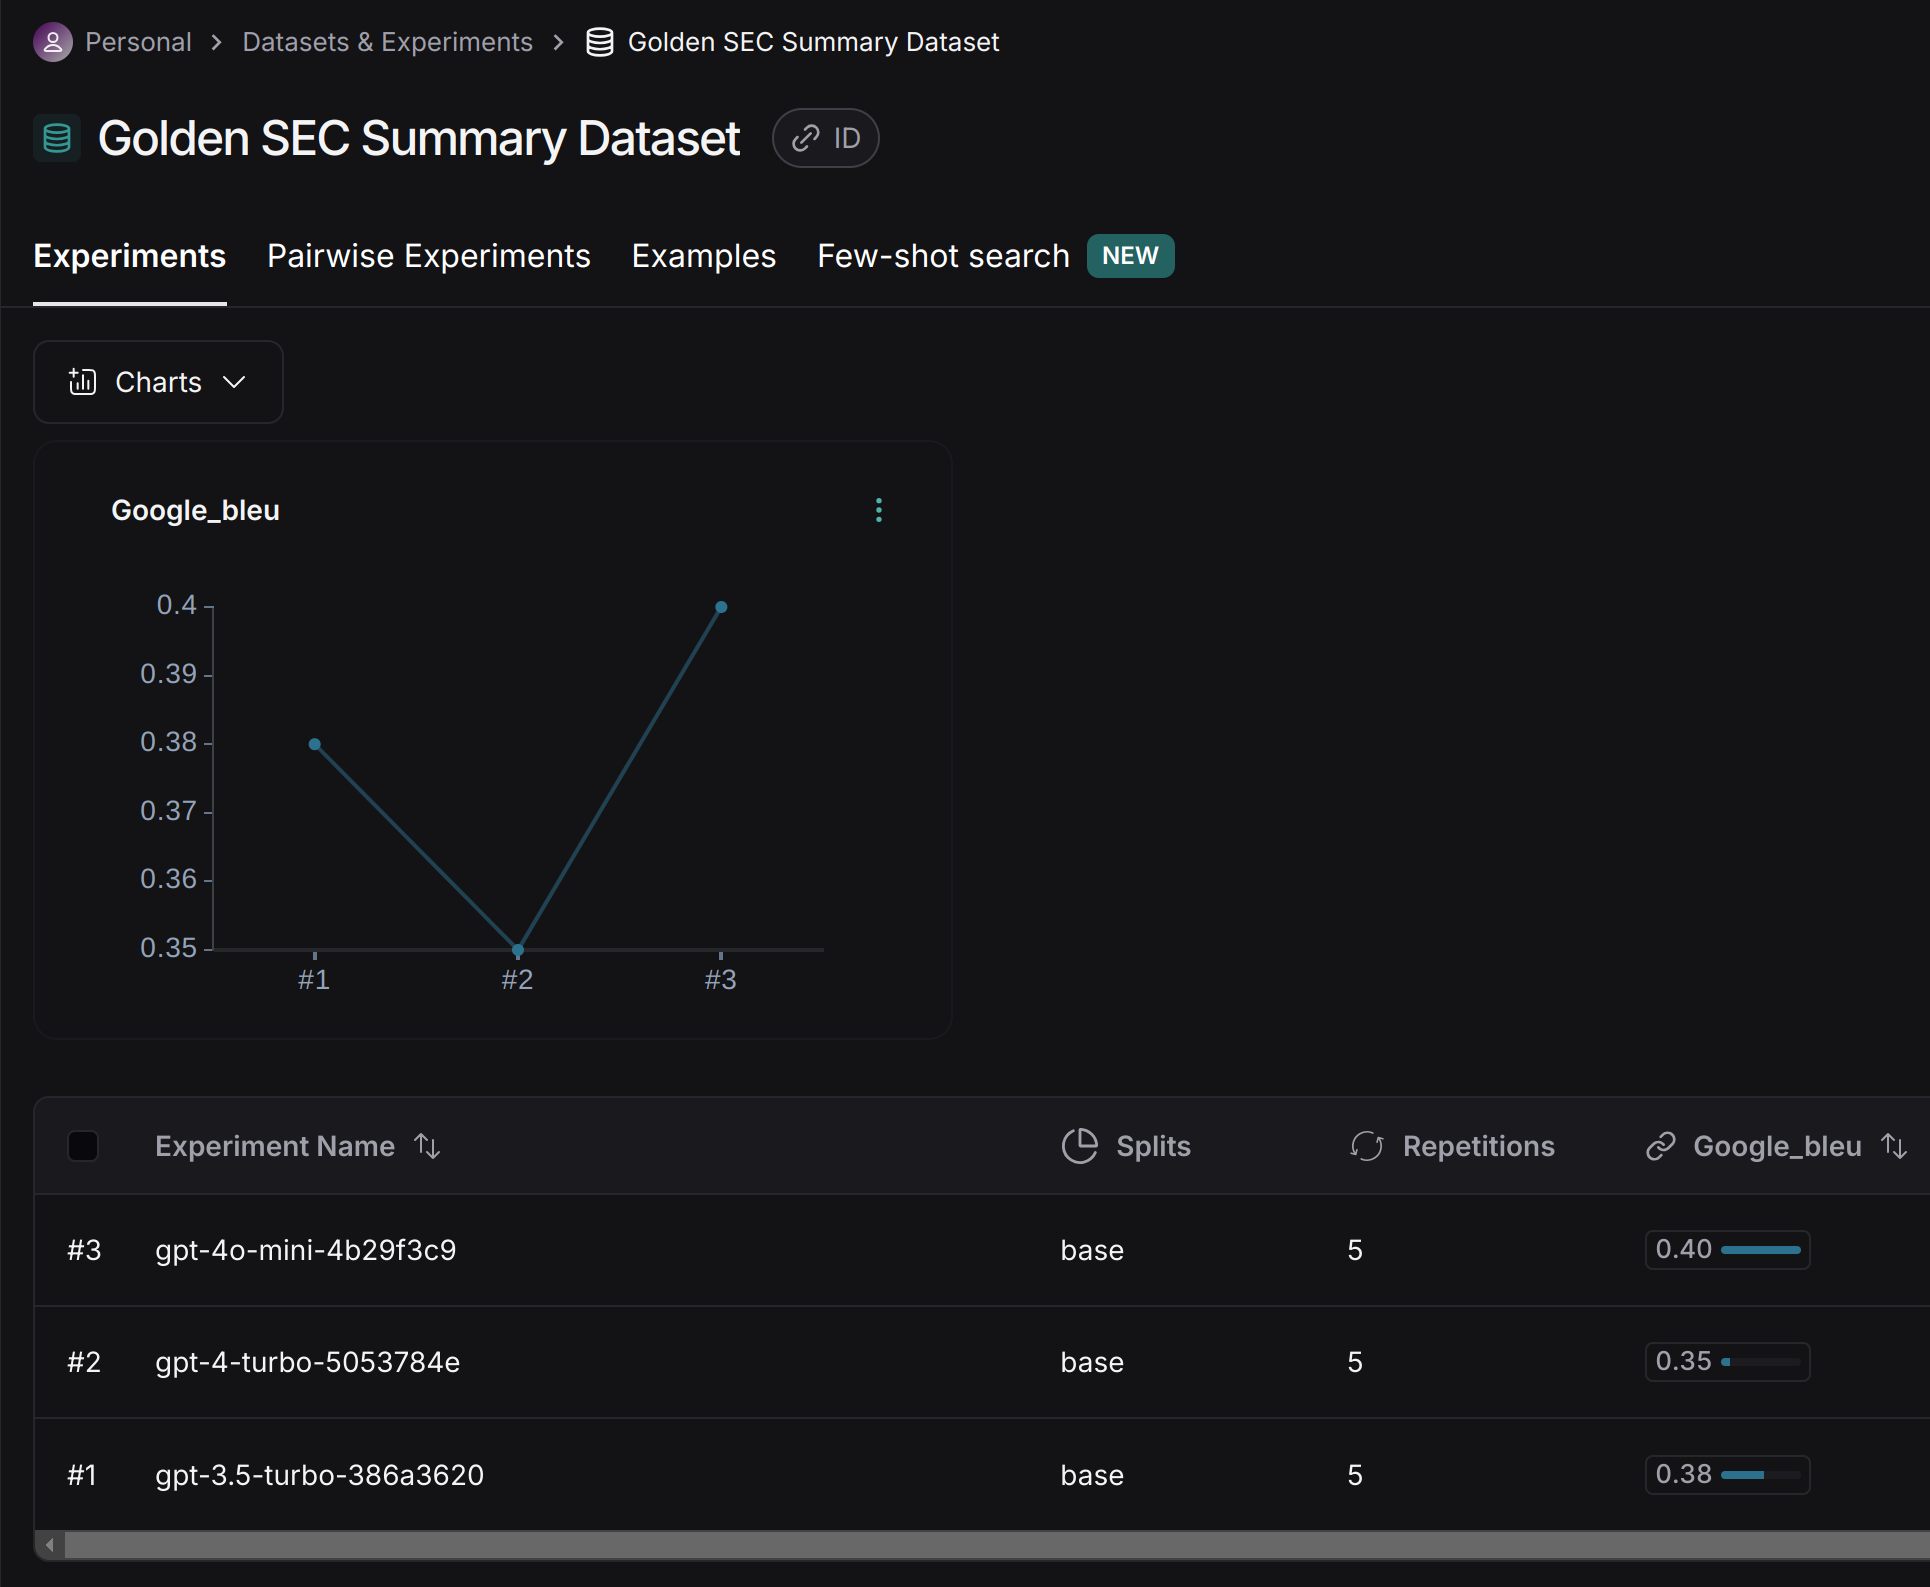
\includegraphics{evals/langsmith.png}
\label{fig:langsmith}
\caption{LangSmith Experiment Results}
\end{figure}
\subsection{PromptFoo}

PromptFoo \sidecite{promptfoo2024} is an open-source framework designed for evaluating applications that utilize LLMs. Key features include:

\begin{enumerate}
    \item \textbf{Automated Testing}: PromptFoo provides automated testing capabilities, allowing developers to run custom evaluations tailored to their applications.

    \item \textbf{Custom Probes}: Developers can create custom probes to focus on specific use cases for instance decoupling prompts from tests cases.

    \item \textbf{User-Friendly CLI}: The framework features a command-line interface that supports live reloads and caching, facilitating rapid testing and iteration.
\end{enumerate}

We will use PromptFoo's command line interface in the following examples. Please follow installation instructions at \url{https://www.promptfoo.dev/docs/installation/#for-command-line-usage}.

Evals are defined in a configuration file \texttt{promptfooconfig.yaml}, which defines elements such as providers, prompts, test cases, and assertions.

In the following example, we will perform a two-step evaluation:

\begin{enumerate}
    \item Evaluate the performance of different LLM models given a set of constraints.
    \item Evaluate the quality of different prompts for the best performing model from 1.
\end{enumerate}


\begin{minted}{python}
import yaml

# Read the YAML file
with open('promptfoo/model_comparison/promptfooconfig.yaml', 'r') as f:
    config = yaml.safe_load(f)

# Pretty print the YAML content 
print(yaml.dump(config, default_flow_style=False, sort_keys=False))
\end{minted}

\begin{minted}{yaml}
description: Best model eval
prompts:
- file://prompt1.txt
providers:
- openai:gpt-4o-mini
- openai:gpt-4
- openai:gpt-3.5-turbo
defaultTest:
  assert:
  - type: cost
    threshold: 0.001
  - type: latency
    threshold: 1000
  - type: python
    value: len(output) < 200
  - type: llm-rubric
    value: Does the summary look like it was written by an expert analyst [Yes/No]?
tests: file://tests.csv
\end{minted}

The configuration file demonstrates PromptFoo's capabilities for evaluating different LLM models. The YAML configuration defines three providers (\texttt{gpt-4o-mini}, \texttt{gpt-4}, and \texttt{gpt-3.5-turbo}) and sets up test assertions to validate their outputs. These assertions check important constraints:

\begin{enumerate}
    \item \textbf{Cost efficiency}: Each inference must cost less than \$0.001
    \item \textbf{Latency requirements}: Response time must be under 1000ms 
    \item \textbf{Output length}: Generated text must be less than 200 characters
    \item \textbf{Output quality}: An LLM-based rubric evaluates if the output appears to be written by an expert (uses \texttt{openai:gpt-4o} model)
\end{enumerate}

The prompts are loaded from an external file (\texttt{prompt1.txt}) and test cases are defined in \texttt{tests.csv}. This structured approach enables systematic evaluation of model performance across multiple decoupled dimensions.

\begin{minted}{bash}
promptfoo eval --no-cache --output eval.json
\end{minted}

This command will run the evaluation and store the results in \texttt{eval.json} while making sure that the evaluation is not cached so we are measuring actual latency of the LLMs. The code below processes the PromptFoo evaluation results stored in \texttt{eval.json}. It reads the evaluation data from the JSON file and extracts key metrics including:

\begin{itemize}
    \item Provider name (e.g. \texttt{gpt-4}, \texttt{gpt-3.5-turbo})
    \item Latency in milliseconds 
    \item Token usage statistics
    \item Cost per request
    \item Number of passed/failed assertions
    \item Prompt token count
    \item Total number of API requests
\end{itemize}

\begin{minted}{python}
import json
import pandas as pd

# Read the JSON file
with open('promptfoo/model_comparison/eval.json', 'r') as f:
    eval_data = json.load(f)

# Extract results into a list of dictionaries
results = []
for prompt in eval_data['results']['prompts']:
    result = {
        'provider': prompt['provider'],
        'latency_ms': prompt['metrics']['totalLatencyMs'],
        'token_usage': prompt['metrics']['tokenUsage']['total'],
        'cost': prompt['metrics']['cost'],
        'assert_pass': prompt['metrics']['assertPassCount'], 
        'assert_fail': prompt['metrics']['assertFailCount'],
        'prompt_tokens': prompt['metrics']['tokenUsage']['prompt'],
        'num_requests': prompt['metrics']['tokenUsage']['numRequests']
    }
    results.append(result)
\end{minted}


\begin{minted}{python}
# Convert to DataFrame
df = pd.DataFrame(results)
print(df)
\end{minted}

\begin{table}[h]
\centering
\begin{tabular}{|l|r|r|r|}
\hline
Variable & openai:gpt-4o-mini & openai:gpt-4 & openai:gpt-3.5-turbo \\
\hline
Latency (ms) & 2463 & 3773 & 1669 \\
Token Usage & 97 & 103 & 95 \\
Cost & \$0.000035 & \$0.004620 & \$0.000091 \\
Assert Pass & 6 & 4 & 7 \\
Assert Fail & 2 & 4 & 1 \\
Prompt Tokens & 52 & 52 & 52 \\
Num Requests & 2 & 2 & 2 \\
\hline
\end{tabular}
\caption{Performance comparison across different OpenAI models}
\label{tab:model-comparison}
\end{table}
The evaluation results reveal interesting performance characteristics across different OpenAI models. \texttt{GPT-3.5-turbo} demonstrates the best overall performance given our criteria with the lowest latency (1669ms), lowest token usage (95), and highest number of passed assertions (7). While \texttt{GPT-4} shows higher token usage (103) and latency (3773ms), it also has the highest cost per request (\$0.00462). The \texttt{GPT-4-mini} variant offers a middle ground, with moderate latency and token usage, while maintaining relatively good assertion performance (6 passes). These results suggest that for this particular evaluation task, \texttt{GPT-3.5-turbo} provides the best balance of performance, reliability, and cost-effectiveness.

Promptfoo also offers a web interface for visualizing the evaluation results as shown in Figure~\ref{fig:promptfoo1}. 

\begin{minted}{bash}
promptfoo view
\end{minted}

We can observe results per test case (i.e. section of the SEC filing) and per provider. Humans can also manually review the results and provide feedback as well as generate new test cases.



\begin{table*}[h]
    \begin{tabular}{lll}
    \hline
    Model Family & Description & Models \\
    \hline
    Llama3.2 Instruct \cite{meta_llama_models} & LLaMA architecture-based \newline pretrained and instruction-tuned \newline generative models & \texttt{Llama-3.2-1B-Instruct} and 
    \texttt{Llama-3.2-3B-Instruct} \\
    \hline
    Qwen2.5 Instruct \cite{gpt2docs,hui2024qwen2,qwen2} & Instruction-tuned LLMs family \newline built by Alibaba Cloud & \texttt{Qwen2.5-0.5B-Instruct}, \texttt{Qwen2.5-1.5B-Instruct} and \texttt{Qwen2.5-3B-Instruct} \\
    \hline
    SmolLM2 Instruct \cite{allal2024SmolLM2}  & Instruction-tuned family of \newline compact language models \newline built by HuggingFace & \texttt{SmolLM2-360M-Instruct} and \texttt{SmolLM2-1.7B-Instruct} \\
    \hline
    \end{tabular}
    \caption{Model Families Evaluated Using LightEval}
    \label{tab:model-families}
    \end{table*}



\begin{figure}[h]
\centering
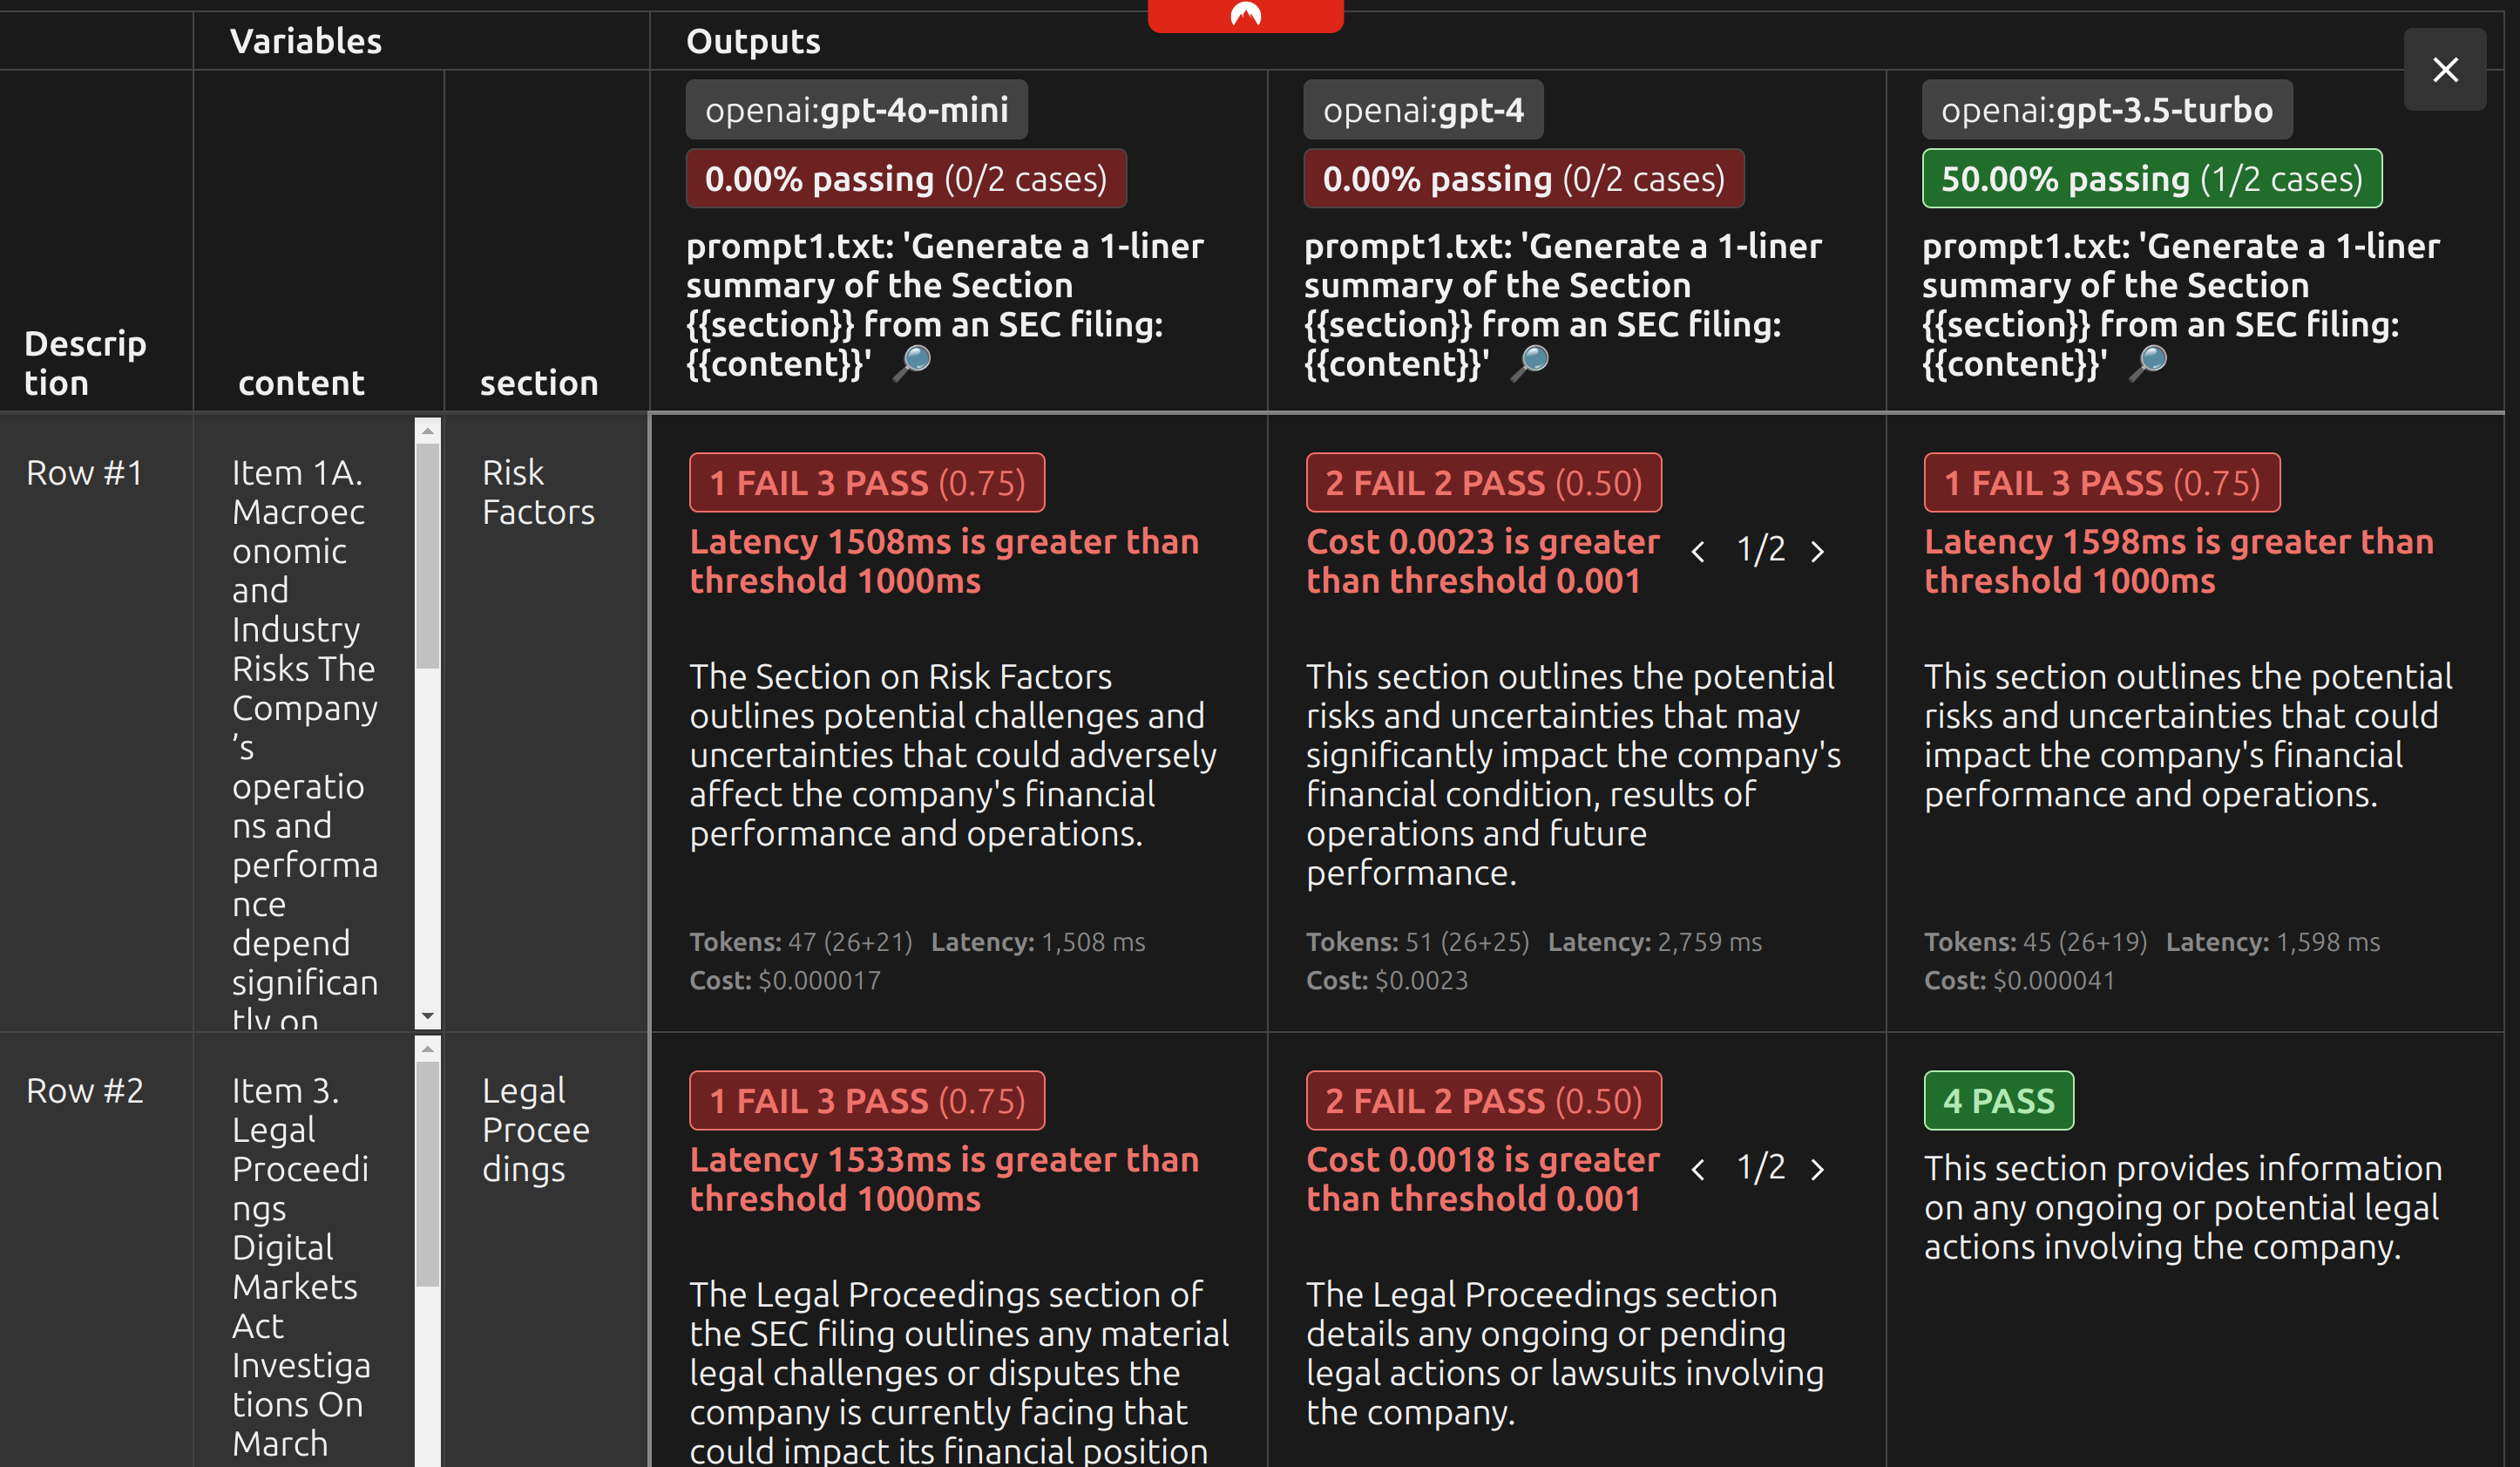
\includegraphics[width=0.3\textwidth]{evals/promptfoo1.png}
\caption{PromptFoo evaluation results showing performance metrics across different models.}
\label{fig:promptfoo1}
\end{figure}

Now that we have established \texttt{GPT-3.5-turbo} as our model of choice given the minimum required criteria based on cost, latency and basic qualitative evaluation, we can compare the performance of different prompts as a next evaluation step. Can we improve the quality of the summaries by using different prompts?

First, we redefine our evaluation criteria. We now would like to select the prompt that delivers the most ``detailed'' summaries. Our updated promptfoo configuration file is shown below.

\begin{minted}{python}
# Read the YAML file
with open('promptfoo/prompt_comparison/promptfooconfig.yaml', 'r') as f:
    config = yaml.safe_load(f)

# Pretty print the YAML content
print(yaml.dump(config, default_flow_style=False, sort_keys=False))
\end{minted}

\begin{minted}{yaml}
description: Best model eval
prompts:
- file://prompt1.txt
- file://prompt2.txt
- file://prompt3.txt
providers:
- openai:gpt-3.5-turbo
defaultTest:
  assert:
  - type: llm-rubric
    value: 'Evaluate the output based on how detailed it is.  Grade it on a scale
      of 0.0 to 1.0, where:

      Score of 0.1: Not much detail.

      Score of 0.5: Some detail.

      Score of 1.0: Very detailed.

      '
tests: file://tests.csv
\end{minted}
    

Note that we are now passing 3 different prompts. And we have updated our assertions to check if the output is ``detailed'' by leveraging promptfoo's \texttt{llm-rubric} assertion which will run an LLM-as-a-Judge for evaluation. Now, let's define 3 prompt variations we would like to test aiming at improving the quality/detail of the summaries.

\begin{minted}{python}
# Display the prompt variations
from IPython.display import display, Markdown

prompt_files = ['prompt1.txt', 'prompt2.txt', 'prompt3.txt']
prompt_content = []

for file in prompt_files:
    with open(f'promptfoo/prompt_comparison/{file}', 'r') as f:
        content = f.read().strip()
        prompt_content.append(f"### {file}\n---\n{content}\n")

display(Markdown("\n\n".join(prompt_content)))
\end{minted}

\begin{verbatim}
### prompt1.txt
---
'Generate a 1-liner summary of the Section {{section}} from an SEC filing: {{content}}'


### prompt2.txt
---
'ROLE: You are a financial analyst. TASK: Generate a 1-liner summary of the Section {{section}} from an SEC filing: {{content}}'


### prompt3.txt
---
'ROLE: You are a financial analyst. REQUIREMENTS: BE DETAILED. TASK: Generate a 1-liner summary of the Section {{section}} from an SEC filing: {{content}}'
\end{verbatim}


The first prompt matches our previous prompt. The second prompt adds a ``financial analyst'' role to the prompt. The third prompt expands on second prompt and add a requirement ``BE DETAILED''.

We can now run the evaluation again.

\begin{minted}{bash}
promptfoo eval --output eval.json
\end{minted}

\begin{minted}{python}
# Read the evaluation results from JSON file
import json
with open('promptfoo/prompt_comparison/eval.json', 'r') as f:
    eval_data = json.load(f)

# Create a list to store the data
data = []

# Extract results for each test case
for result in eval_data['results']['results']:
    section = result['vars']['section']
    prompt_id = result['promptId']
    score = result['gradingResult']['score'] if 'gradingResult' in result else 0.0
    
    # Find the corresponding prompt file
    for prompt in eval_data['results']['prompts']:
        if prompt['id'] == prompt_id:
            prompt_file = prompt['label'].split(':')[0]
            break
            
    # Add to data list
    data.append([section, prompt_file, score])

# Convert to DataFrame
df_raw = pd.DataFrame(data, columns=['Section', 'Prompt', 'Score'])

# Pivot to get desired format
df = df_raw.pivot(index='Section', columns='Prompt', values='Score').reset_index()
df = df[['Section', 'prompt1.txt', 'prompt2.txt', 'prompt3.txt']]

display(Markdown("### Prompt Comparison Results by Section"))
print(df)
\end{minted}

\begin{table}[h]
\centering
\begin{tabular}{lccc}
\hline
Section & prompt1.txt & prompt2.txt & prompt3.txt \\
\hline
Legal Proceedings & 0.1 & 0.5 & 1.0 \\
Risk Factors & 0.1 & 0.5 & 0.5 \\
\hline
\end{tabular}
\end{table}

The results demonstrate that \texttt{prompt3.txt} exhibits superior performance for Legal Proceedings sections, attaining a perfect score of 1.0 compared to 0.5 for \texttt{prompt2.txt} and 0.1 for \texttt{prompt1.txt}. For Risk Factors sections, both \texttt{prompt2.txt} and \texttt{prompt3.txt} achieve moderate scores of 0.5, while \texttt{prompt1.txt} performs poorly with 0.1. This analysis suggests that \texttt{prompt3.txt} demonstrates greater effectiveness at extracting detailed information, particularly for legal content. The findings indicate that defining a Role and specifying requirements for detailed output serves as an effective approach to enhance summary quality, at least within the constraints of this specific task, model, and evaluation criteria.

In conclusion, Promptfoo demonstrates its value as an effective LLM application evaluation tool, particularly through its capacity to decouple various components of the evaluation process. This decoupling enables users to concentrate on the most critical aspects of evaluation based on their specific application requirements and criteria, establishing Promptfoo as a versatile and valuable tool for LLM application development.

\subsection{Comparison}

Table~\ref{tab:tool-comparison} presents a comparative analysis of three open source frameworks for language models evaluation discussed: Lighteval, LangSmith, and Promptfoo. Each framework undergoes assessment based on key features including integration capabilities, customization options, ease of use, and the ability to facilitate human and LLM collaboration.
\begin{table}[h]
\centering
\begin{tabular}{lp{3cm}p{3cm}p{3cm}}
\hline
\textbf{Feature/Aspect} & \textbf{Lighteval} & \textbf{LangSmith} & \textbf{Promptfoo} \\
\hline
\textbf{Integration} & Seamless with Hugging Face models, easy access to multiple inference engines, and remote evaluation (e.g., TGI servers, HF serverless models) & User-provided models, evaluators, and metrics & CLI-based, user-provided models via YAML \\
\hline
\textbf{Customization} & Flexible task and metric support, quick evaluation against state-of-the-art leaderboards & Easy setup of custom tasks and metrics with plain vanilla Python functions, lacks predefined tasks and metrics & Default and user-provided probes, metrics, and assertions \\
\hline
\textbf{Ease of Use} & User-friendly, minimal setup & User-friendly, minimal setup, includes UI for result visualization & Simple CLI, rapid testing, includes UI for result visualization \\
\hline
\textbf{Human/LLM Collaboration} & Model-based evaluation & Model-based evaluation & Supports human and model evaluators \\
\hline
\end{tabular}
\caption{Comparison of Lighteval, LangSmith, and Promptfoo}
\label{tab:tool-comparison}
\end{table}

\section{Conclusion}

Language models have fundamentally transformed how software is developed and evaluated. Unlike conventional systems that produce predictable outputs, LLMs generate varied, probabilistic responses that defy traditional testing approaches. While developers accustomed to deterministic systems may find this shift challenging, continuing to rely on legacy testing methods is unsustainable. These frameworks were not designed to handle the inherent variability of LLM outputs and will ultimately prove inadequate.

Success requires embracing this new paradigm by implementing comprehensive evals that cover the non-deterministic generative nature of LLMs - this is the new Product Requirements Document (PRD) - and cultivating an organizational mindset focused on iteration, experimentation and growth.

The shift from traditional software testing to LLM evaluation is not just a change in tools but a transformation in mindset. Those who recognize and adapt to this shift will lead the way in harnessing the power of LLMs in software development.
